\documentclass[aspectratio=169, 11pt]{beamer}

% ── Theme & colours ──────────────────────────────────────────────
\usetheme{Madrid}
\usecolortheme{seahorse}
\setbeamertemplate{navigation symbols}{}
\setbeamertemplate{itemize items}[circle]

\newcommand{\mainend}{0}
\setbeamertemplate{footline}{%
  \hfill%
  \usebeamerfont{footline}%
  \insertframenumber\,/\,\mainend%
  \hspace*{4pt}\vskip4pt%
}

% ── Packages ─────────────────────────────────────────────────────
\usepackage{amsmath,amssymb}
\usepackage{graphicx}
\usepackage{booktabs}
\usepackage{xcolor}
\usepackage{colortbl}
\usepackage{tikz}
\usetikzlibrary{arrows.meta, positioning, shapes.geometric, fit, backgrounds, calc}

% ── Macros ───────────────────────────────────────────────────────
\newcommand{\bh}{black hole}
\newcommand{\BH}{Black Hole}
\newcommand{\pinn}{PINN}
\newcommand{\pinns}{PINNs}
\newcommand{\qnm}{QNM}
\newcommand{\qnms}{QNMs}
\newcommand{\fd}{FD}
\newcommand{\rw}{Regge--Wheeler}
\newcommand{\zer}{Zerilli}

\definecolor{darkgreen}{rgb}{0.0, 0.5, 0.0}
\definecolor{darkred}{rgb}{0.7, 0.0, 0.0}

% ── Title ────────────────────────────────────────────────────────
\title[QNMs with PINNs --- Onboarding]{Computing Quasi-Normal Modes\\of Schwarzschild Black Holes\\with Physics-Informed Neural Networks}
\subtitle{Project Onboarding Walkthrough}
\author{Jonathan Chung}
\institute{University of Cambridge}
\date{\today}

\begin{document}

\begin{frame}\titlepage\end{frame}

\begin{frame}{Outline}\tableofcontents\end{frame}


% ══════════════════════════════════════════════════════════════════
\section{1. Introduction \& Background}
% ══════════════════════════════════════════════════════════════════

\begin{frame}{The physical picture --- black-hole ringdown}
  \begin{columns}[T]
    \begin{column}{0.55\textwidth}
      A perturbed Schwarzschild \bh{} ``rings'' like a struck bell:
      after the merger, the geometry settles down by emitting
      \textbf{damped sinusoidal} gravitational waves --- the
      \textbf{Quasi-Normal Modes (\qnms{})}.
      \medskip
      \[
        h(t) \;\propto\; e^{-t/\tau}\cos(\omega\, t + \phi_0)
      \]
      \begin{itemize}\small
        \item $\omega$ --- ringing frequency (real part).
        \item $\tau = -1/\Im\omega$ --- damping time (imaginary part).
        \item Determined entirely by the \bh{}'s mass $M$ and spin $a$.
        \item Observed by LIGO/Virgo in every binary-\bh{} detection
              since GW150914.
      \end{itemize}
    \end{column}
    \begin{column}{0.42\textwidth}
      \centering
      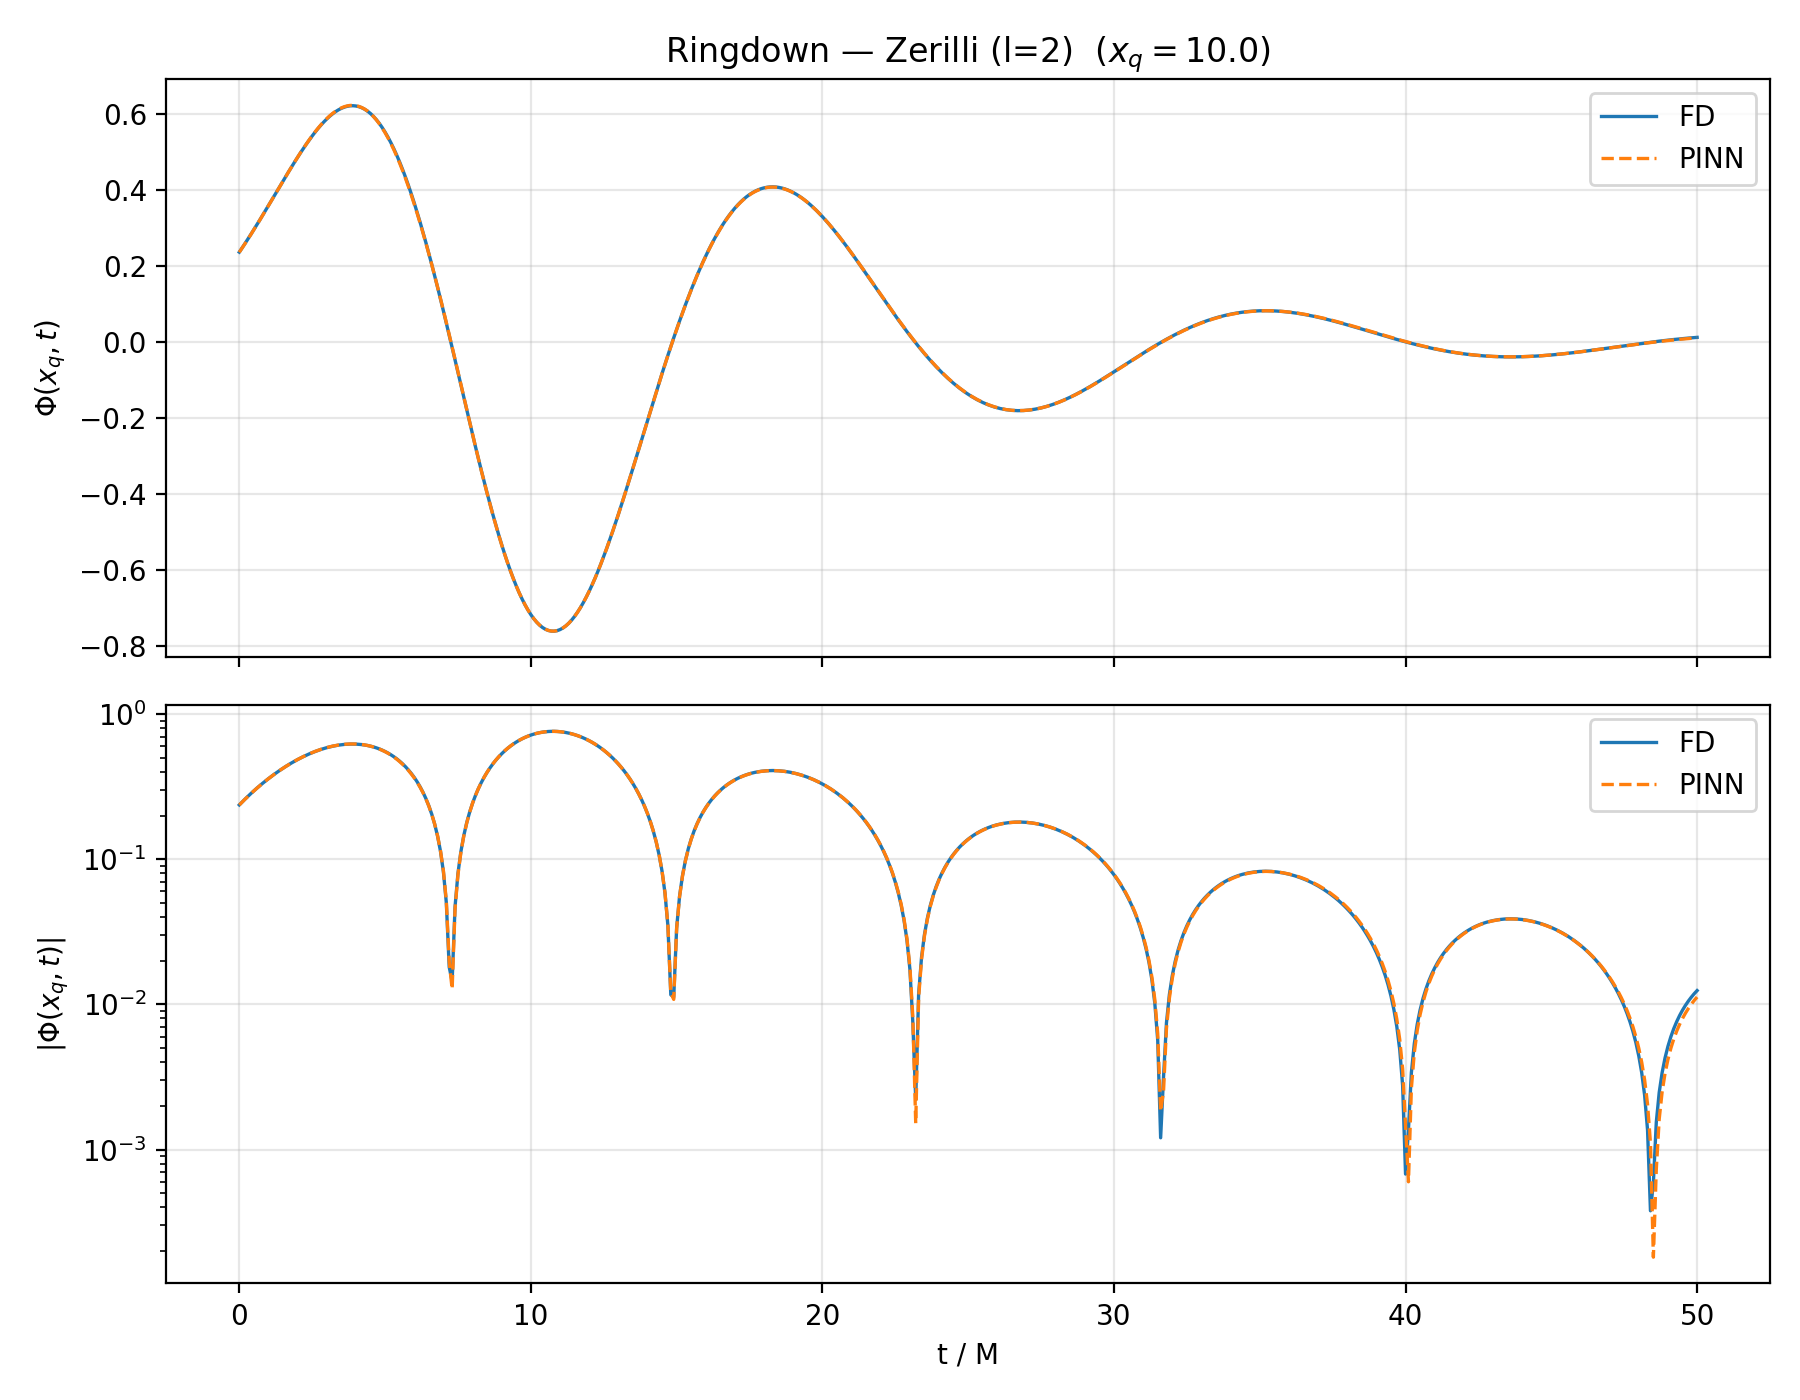
\includegraphics[width=\textwidth]{../outputs/pinn/zerilli_l2_greedy_f03_lbfgs30k/ringdown_overlay.png}
      \\{\footnotesize Ringdown waveform $\Phi(x_q\!=\!10M,\,t)$}
    \end{column}
  \end{columns}
\end{frame}

% ── Theory frame 1: Schwarzschild + linearised perturbations ─────
\begin{frame}{From Einstein's equations to a 1+1D wave problem}
  \textbf{Step 1 --- background.} Schwarzschild geometry ($M$ is the \bh{} mass),
  \[
    \mathrm{d} s^{2} \;=\; -f(r)\,\mathrm{d} t^{2} + f(r)^{-1}\mathrm{d} r^{2}
                     + r^{2}\,\mathrm{d}\Omega^{2},
    \qquad f(r) = 1 - \tfrac{2M}{r}.
  \]

  \textbf{Step 2 --- linear perturbation.} Write
  $g_{\mu\nu} = g^{(0)}_{\mu\nu} + h_{\mu\nu}$ with $|h| \ll |g^{(0)}|$ and
  expand the vacuum Einstein equations to first order:
  \[
    \delta R_{\mu\nu}[h] \;=\; 0 .
  \]

  \textbf{Step 3 --- exploit spherical symmetry.} Decompose $h_{\mu\nu}$ in
  \emph{tensor spherical harmonics}; under $(\theta,\varphi)\!\to\!(\pi-\theta,\varphi+\pi)$
  the modes split into two \textbf{decoupled parity sectors}:
  \medskip
  \begin{center}\small
  \begin{tabular}{lll}
    \toprule
    Sector & Parity & Master equation \\ \midrule
    \textbf{Axial} (odd) & $(-1)^{\ell+1}$ & \rw{} \\
    \textbf{Polar} (even)& $(-1)^{\ell}$   & \zer{} \\
    \bottomrule
  \end{tabular}
  \end{center}
  \medskip
  Each sector reduces to a single scalar field $\Phi(t,r_{\!*})$ on the
  \textbf{tortoise coordinate} $\mathrm{d} r_{\!*} = \mathrm{d} r/f(r)$.
\end{frame}


% ── Theory frame 2: the two master equations side by side ────────
\begin{frame}{The two master equations --- \rw{} and \zer{}}
  Both sectors obey the \textbf{same 1+1D wave form}
  \[
    -\,\frac{\partial^{2}\Phi}{\partial t^{2}}
    \;+\; \frac{\partial^{2}\Phi}{\partial r_{\!*}^{\,2}}
    \;-\; V_{\ell}(r)\,\Phi \;=\; 0 ,
  \]
  but with two \emph{different} effective potentials:
  \medskip
  \begin{columns}[T]
    \begin{column}{0.42\textwidth}
      \centering\textbf{\rw{} (axial)}\par\medskip
      \[
        V^{\mathrm{RW}}_{\ell}(r) = f(r)\!\left[\frac{\ell(\ell{+}1)}{r^{2}} - \frac{6M}{r^{3}}\right]
      \]
    \end{column}
    \begin{column}{0.56\textwidth}
      \centering\textbf{\zer{} (polar)}\par\medskip
      \[
        V^{\mathrm{Z}}_{\ell}(r) = f(r)\,\frac{2\bigl[n^{2}(n{+}1)r^{3}+3n^{2}Mr^{2}+9nM^{2}r+9M^{3}\bigr]}{r^{3}(nr+3M)^{2}}
      \]
      {\centering\scriptsize $n = \tfrac{1}{2}(\ell-1)(\ell+2)$.\par}
    \end{column}
  \end{columns}
  \vfill
  \footnotesize
  Two \emph{different} potentials, one for each parity sector --- but as we
  will see on the next slide, they encode \emph{the same physics}.
\end{frame}


% ── Theory frame 2b: isospectrality (plot + statement) ───────────
\begin{frame}{Isospectrality --- one spectrum, two potentials}
  \begin{columns}[T]
    \begin{column}{0.55\textwidth}
      \centering
      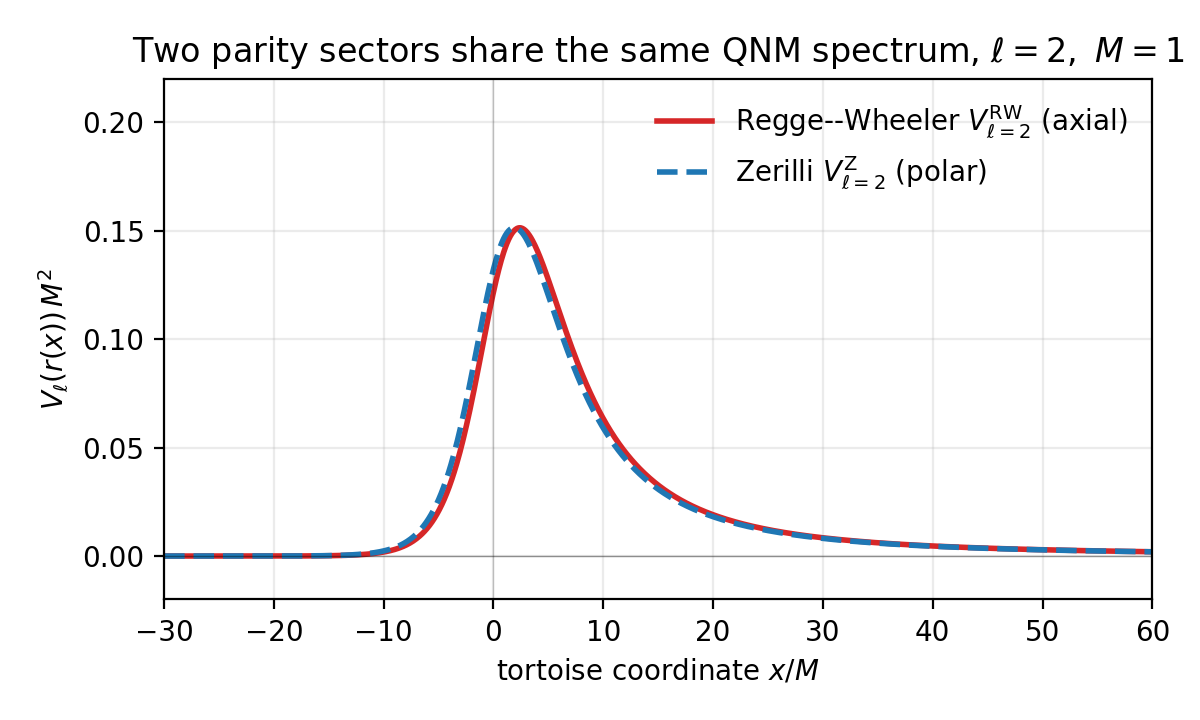
\includegraphics[width=\textwidth]{../outputs/background/rw_vs_zerilli_l2.png}
    \end{column}
    \begin{column}{0.43\textwidth}
      \footnotesize
      \textbf{Chandrasekhar--Detweiler isospectrality:} the two
      potentials are \emph{distinct} but share \emph{exactly the same}
      \qnm{} spectrum $\{\omega_{n}\}$.
      \medskip

      $\Rightarrow$ Either equation is a valid target for our solver.
      \medskip

      This work uses the \textbf{\zer{} (polar, $\ell\!=\!2$)} form,
      matching the reference PINN literature (Patel \emph{et al.}\ 2024)
      and giving a single, well-defined benchmark to push accuracy
      against.
    \end{column}
  \end{columns}
\end{frame}


% ── Theory frame 3: BCs, IC, reference QNM ───────────────────────
\begin{frame}{The numerical problem we actually solve}
  Target: the polar $\ell\!=\!2$ \zer{} equation on
  $r_{\!*}/M \in [-50,\,150]$, $t/M \in [0,\,50]$.
  \medskip
  \begin{itemize}
    \item \textbf{Initial condition} ($t=0$): localised Gaussian pulse,
          time-symmetric ($\partial_{t}\Phi = 0$).
    \item \textbf{Boundary conditions:}
          \emph{purely outgoing} waves at $r_{\!*}\!\to\!+\infty$
          (radiation to infinity),
          \emph{purely ingoing} at $r_{\!*}\!\to\!-\infty$
          (absorption by the horizon).
    \item These BCs are precisely what selects the discrete
          \textbf{\qnm{} spectrum} $\omega_{n}\in\mathbb{C}$.
  \end{itemize}
  \medskip
  \textbf{Reference fundamental mode} ($\ell\!=\!2,\,n\!=\!0$, Leaver 1985):
  \[
    M\omega \;=\; 0.3737 - 0.0890\,i,
    \qquad \tau/M \;=\; -1/\Im\omega \;=\; 11.241 .
  \]
  Every result in the rest of the talk is benchmarked against this number.
\end{frame}

\begin{frame}{Three ways to compute \qnms{}}
  \footnotesize
  \begin{block}{1.\ Leaver continued fraction (1985) --- the \emph{exact reference}}
    Frobenius series ansatz $\Rightarrow$ 3-term recurrence
    $\Rightarrow$ Pincherle continued fraction. \\
    \textbf{+} 12-digit accuracy in milliseconds.
    \quad \textbf{--} only works on known analytic potentials.
  \end{block}
  \begin{block}{2.\ Finite-difference (\fd{}) time evolution --- the \emph{ground truth waveform}}
    2nd-order centred FD on the $(r_{\!*}, t)$ grid;
    extract $\omega,\tau$ from the late-time signal. \\
    \textbf{+} produces the full $(x,t)$ field used to train our PINN.
    \quad \textbf{--} slow.
  \end{block}
  \begin{block}{3.\ Physics-Informed Neural Network (\pinn{}) --- our tool}
    NN $\Phi_{\theta}(x,t)$ trained to satisfy PDE $+$ IC $+$ BC. \\
    \textbf{+} mesh-free, differentiable, jointly learns physical parameters.
    \quad \textbf{--} slower and less accurate than Leaver/\fd{} on Schwarzschild.
  \end{block}
\end{frame}

\begin{frame}{Why bother with PINNs at all on Schwarzschild?}
  \begin{itemize}
    \item Schwarzschild is the \textbf{controlled benchmark}: every answer
          is known to 12 digits, so any PINN error is \emph{measurable}.
    \item PINNs are \textbf{differentiable end-to-end}: the same training
          loop can solve the \emph{inverse} problem (recover $M, \omega, \tau$
          from data).
    \item Patel et al.\ 2024 introduced PINNs for \qnms{} but report only
          $\sim$1--2 digit accuracy.
    \item \textbf{Our work pushes this methodology into a regime where it
          actually competes} with classical extractors.
  \end{itemize}
\end{frame}

\begin{frame}{What this project actually contributes}
  Schwarzschild $\ell\!=\!2$ is the \textbf{stress test} for QNM-PINNs ---
  every error is measurable against an exact reference. Our contributions:
  \medskip
  \begin{enumerate}
    \item \textbf{Forward PINN, accuracy push:} hard boundary conditions,
          gPINN residuals, \textbf{greedy adaptive sampling},
          extended L-BFGS. Pushes spatial RMSD down by $\sim$$55\%$ vs.\
          uniform sampling and $\omega$ error to $0.03\%$.
    \medskip
    \item \textbf{Inverse PINN:} learn $M,\omega,\tau$ from ringdown data
          in a single training run. Best variant (\textbf{D\_combo}): $M$ to $0.34\%$,
          $\omega$ to $0.31\%$, $\tau$ to $1.6\%$.
    \medskip
    \item \textbf{Curriculum PINN:} split $t\!\in\![0,50]M$ into
          $K$ windows trained sequentially, IC of window $k$ taken
          from network $k\!-\!1$. Diagnoses where the late-time
          error of the single-window forward PINN comes from.
    \medskip
    \item \textbf{New extraction methodology --- M3, M4, M5:}
          ESPRIT subspace decomposition; two-mode NLS with 1-D and 2-D
          \emph{plateau scans} to give principled, falsifiable
          $(\omega, \tau)$ estimates with systematic-error bars.
    \medskip
    \item \textbf{Greedy resampling:} simple, deterministic, hyperparameter-light
          replacement for RAD with measurably better accuracy.
  \end{enumerate}
\end{frame}


% ══════════════════════════════════════════════════════════════════
\section{2. Forward PINN}
% ══════════════════════════════════════════════════════════════════

\begin{frame}{Forward PINN --- problem statement}
  \textbf{Goal.} Train a neural network
  $\Phi_{\boldsymbol{\theta}}(x,t)$ to satisfy the Zerilli PDE on the
  full $(x,t)$ domain, plus its initial and boundary conditions.
  \bigskip

  We minimise a sum of \textbf{seven} weighted mean-squared-error terms,
  \[
    \mathcal{L}_{\text{fwd}}(\boldsymbol{\theta})
    \;=\;
    \underbrace{\textcolor{darkred}{\lambda_{r}\mathcal{L}_{r}
      + \lambda_{r_x}\mathcal{L}_{r_x}
      + \lambda_{r_t}\mathcal{L}_{r_t}}}_{\text{PDE residual + gPINN}}
    \;+\;
    \underbrace{\textcolor{darkgreen}{\lambda_{ic}\mathcal{L}_{ic}
      + \lambda_{iv}\mathcal{L}_{iv}}}_{\text{initial condition at }t=0}
    \;+\;
    \underbrace{\textcolor{blue}{\lambda_{bl}\mathcal{L}_{bl}
      + \lambda_{br}\mathcal{L}_{br}}}_{\text{boundary conditions}}
  \]
  \bigskip

  Each $\mathcal{L}_i$ is a mean of squared residuals over a sample of
  collocation points; the next two slides write out all seven sums
  explicitly.
\end{frame}

\begin{frame}{Forward PINN loss --- PDE residual $+$ gPINN}
  \footnotesize
  Define the \textbf{PDE residual} of the Zerilli equation,
  \[
    r_{\theta}(x,t) \;\equiv\;
    -\,\partial_{t}^{2}\Phi_{\theta}(x,t)
    \;+\; \partial_{x}^{2}\Phi_{\theta}(x,t)
    \;-\; V_{\ell}(r)\,\Phi_{\theta}(x,t).
  \]
  At $N_{r}=32{,}000$ randomly drawn collocation points
  $\{(x_{i},t_{i})\}_{i=1}^{N_{r}}$ inside the domain we evaluate
  three mean-squared losses:
  \medskip
  \[
    \textcolor{darkred}{\mathcal{L}_{r}}
      \;=\; \frac{1}{N_{r}}\sum_{i=1}^{N_{r}}
            \bigl[\,r_{\theta}(x_{i},t_{i})\,\bigr]^{2}
    \qquad\text{(standard PINN residual)}
  \]
  \[
    \textcolor{darkred}{\mathcal{L}_{r_{x}}}
      \;=\; \frac{1}{N_{r}}\sum_{i=1}^{N_{r}}
            \bigl[\,\partial_{x} r_{\theta}(x_{i},t_{i})\,\bigr]^{2},
    \qquad
    \textcolor{darkred}{\mathcal{L}_{r_{t}}}
      \;=\; \frac{1}{N_{r}}\sum_{i=1}^{N_{r}}
            \bigl[\,\partial_{t} r_{\theta}(x_{i},t_{i})\,\bigr]^{2}
  \]
  \medskip
  The two extra terms are the \textbf{gPINN} regularisers of
  Yu \emph{et al.} 2022: penalising the gradient of the residual
  forces the residual to be \emph{smoothly} small, not just
  point-wise small, and gives noticeably cleaner derivatives.
\end{frame}

\begin{frame}{Forward PINN loss --- initial and boundary conditions}
  \footnotesize
  \textcolor{darkgreen}{\textbf{Initial condition} at $t=0$}, on
  $N_{\mathrm{ic}}$ points $\{x_{j}\}_{j=1}^{N_{\mathrm{ic}}}$ along
  the spatial axis:
  \[
    \textcolor{darkgreen}{\mathcal{L}_{\mathrm{ic}}}
      \;=\; \frac{1}{N_{\mathrm{ic}}}\sum_{j=1}^{N_{\mathrm{ic}}}
            \bigl[\,\Phi_{\theta}(x_{j},0)-\Phi_{0}(x_{j})\,\bigr]^{2}
    \qquad\Phi_{0}(x)\text{ is a Gaussian pulse},
  \]
  \[
    \textcolor{darkgreen}{\mathcal{L}_{\mathrm{iv}}}
      \;=\; \frac{1}{N_{\mathrm{ic}}}\sum_{j=1}^{N_{\mathrm{ic}}}
            \bigl[\,\partial_{t}\Phi_{\theta}(x_{j},0)\,\bigr]^{2}
    \qquad\text{(time-symmetric initial data)}.
  \]
  \medskip
  \textcolor{blue}{\textbf{Boundary conditions}}, on
  $N_{\mathrm{bc}}$ time points $\{t_{k}\}_{k=1}^{N_{\mathrm{bc}}}$ at each
  domain edge --- outgoing waves at $x_{\max}$, ingoing at $x_{\min}$:
  \[
    \textcolor{blue}{\mathcal{L}_{\mathrm{bl}}}
      \;=\; \frac{1}{N_{\mathrm{bc}}}\sum_{k=1}^{N_{\mathrm{bc}}}
            \bigl[\,(\partial_{t}-\partial_{x})\Phi_{\theta}(x_{\min},t_{k})\,\bigr]^{2},
  \]
  \[
    \textcolor{blue}{\mathcal{L}_{\mathrm{br}}}
      \;=\; \frac{1}{N_{\mathrm{bc}}}\sum_{k=1}^{N_{\mathrm{bc}}}
            \bigl[\,(\partial_{t}+\partial_{x})\Phi_{\theta}(x_{\max},t_{k})\,\bigr]^{2}.
  \]
\end{frame}

\begin{frame}{Forward PINN --- training setup}
  \begin{itemize}
    \item \textbf{Network.} Fully-connected MLP with layer widths
          $[\,2,80,40,20,10,1\,]$, $\tanh$ activations
          ($\sim\!4{,}500$ trainable parameters).
    \item \textbf{Output transform.}
          $\Phi_{\theta}(x,t) = A\,\tanh\!\bigl(\,\widetilde{\Phi}_{\theta}(x,t)\,\bigr)$
          with $A=1$, where $\widetilde{\Phi}_{\theta}$ is the raw network
          output. This bounds the field and stabilises early training.
    \item \textbf{Loss weights.}
          $\boldsymbol{\lambda} =
            (\lambda_{r},\lambda_{r_{x}},\lambda_{r_{t}},
             \lambda_{\mathrm{ic}},\lambda_{\mathrm{iv}},
             \lambda_{\mathrm{bl}},\lambda_{\mathrm{br}})
          = (100,\,100,\,100,\,1,\,100,\,1,\,1)$.
    \item \textbf{Optimiser.} Adam for $10{,}000$ steps to find a good
          basin, then \textbf{L-BFGS} for $30{,}000$ steps to converge
          inside it.
    \item \textbf{Sampling.} Collocation points are re-drawn every
          epoch via the \emph{greedy resampling} scheme described in
          \S 6.
  \end{itemize}
\end{frame}

\begin{frame}{Forward PINN --- our architecture}
  \centering
  \resizebox{0.95\textwidth}{!}{%
  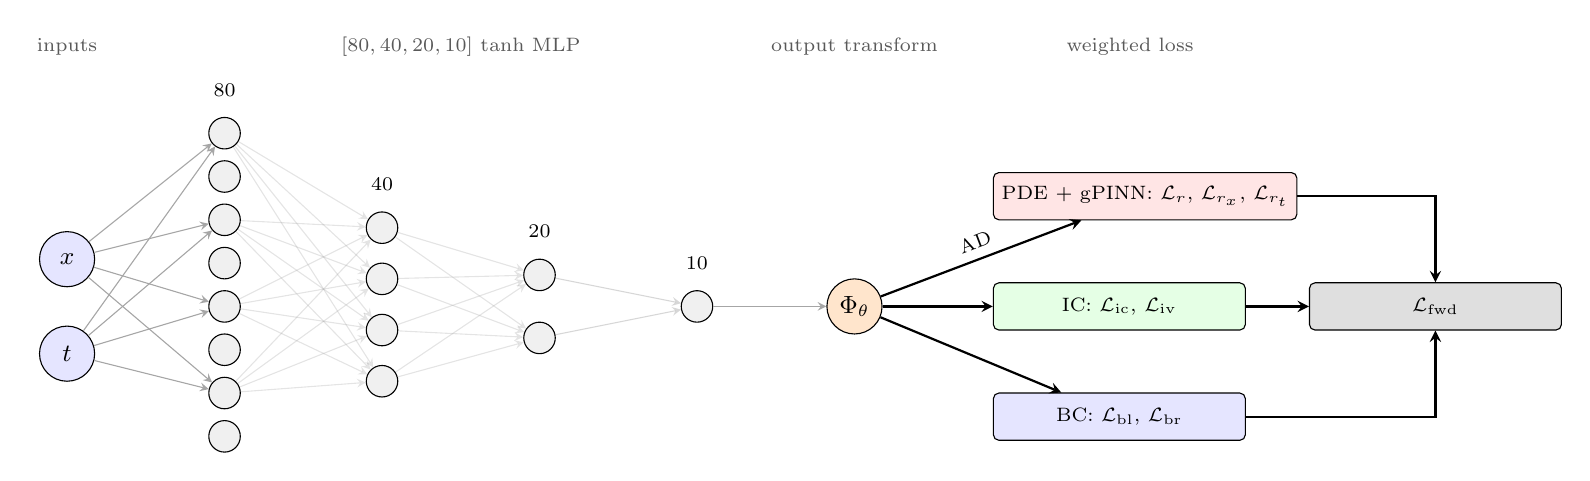
\begin{tikzpicture}[
    node distance=10mm and 12mm,
    every node/.style={font=\small},
    inp/.style={circle, draw, fill=blue!10, minimum size=7mm, inner sep=0pt},
    hid/.style={circle, draw, fill=gray!12, minimum size=4mm, inner sep=0pt},
    outn/.style={circle, draw, fill=orange!20, minimum size=7mm, inner sep=0pt},
    loss/.style={rectangle, draw, fill=green!10, rounded corners=2pt,
                 minimum height=6mm, minimum width=32mm, inner sep=3pt,
                 align=center, font=\scriptsize},
    arr/.style={->, >=stealth, thin, gray!70},
  ]
    \node[inp] (x) at (0, 0) {$x$};
    \node[inp] (t) at (0, -1.2) {$t$};
    \def\xL{2.0}\def\xLii{4.0}\def\xLiii{6.0}\def\xLiv{8.0}
    \foreach \k/\y in {1/1.6, 2/1.05, 3/0.5, 4/-0.05, 5/-0.6, 6/-1.15, 7/-1.7, 8/-2.25}{
      \node[hid] (a\k) at (\xL, \y) {};}
    \foreach \k/\y in {1/0.4, 2/-0.25, 3/-0.9, 4/-1.55}{
      \node[hid] (b\k) at (\xLii, \y) {};}
    \foreach \k/\y in {1/-0.2, 2/-1.0}{
      \node[hid] (c\k) at (\xLiii, \y) {};}
    \node[hid] (d1) at (\xLiv, -0.6) {};
    \node[font=\scriptsize] at (\xL, 2.15) {$80$};
    \node[font=\scriptsize] at (\xLii, 0.95) {$40$};
    \node[font=\scriptsize] at (\xLiii, 0.35) {$20$};
    \node[font=\scriptsize] at (\xLiv, -0.05) {$10$};
    \node[outn] (phi) at (10.0, -0.6) {$\Phi_\theta$};
    \foreach \src in {x, t}\foreach \dst in {a1, a3, a5, a7}\draw[arr] (\src) -- (\dst);
    \foreach \a in {1,3,5,7}\foreach \b in {1,2,3,4}\draw[arr, opacity=0.30] (a\a) -- (b\b);
    \foreach \a in {1,2,3,4}\foreach \b in {1,2}\draw[arr, opacity=0.30] (b\a) -- (c\b);
    \foreach \a in {1,2}\draw[arr, opacity=0.45] (c\a) -- (d1);
    \draw[arr] (d1) -- (phi);
    \node[loss, fill=red!10, right=14mm of phi, yshift=14mm] (lpde)
      {PDE + gPINN: $\mathcal{L}_{r},\,\mathcal{L}_{r_x},\,\mathcal{L}_{r_t}$};
    \node[loss, fill=green!10, right=14mm of phi] (lic)
      {IC: $\mathcal{L}_{\mathrm{ic}},\,\mathcal{L}_{\mathrm{iv}}$};
    \node[loss, fill=blue!10, right=14mm of phi, yshift=-14mm] (lbc)
      {BC: $\mathcal{L}_{\mathrm{bl}},\,\mathcal{L}_{\mathrm{br}}$};
    \draw[arr, thick, black] (phi) -- (lpde) node[midway, above, font=\scriptsize, sloped] {AD};
    \draw[arr, thick, black] (phi) -- (lic);
    \draw[arr, thick, black] (phi) -- (lbc);
    \node[loss, fill=gray!25, right=8mm of lic] (ltot)
      {$\mathcal{L}_{\mathrm{fwd}}$};
    \draw[arr, thick, black] (lpde) -| (ltot);
    \draw[arr, thick, black] (lic) -- (ltot);
    \draw[arr, thick, black] (lbc) -| (ltot);
    \node[font=\scriptsize, gray!70!black] at (0.0, 2.7) {inputs};
    \node[font=\scriptsize, gray!70!black] at (5.0, 2.7) {$[80,40,20,10]$ tanh MLP};
    \node[font=\scriptsize, gray!70!black] at (10.0, 2.7) {output transform};
    \node[font=\scriptsize, gray!70!black] at (13.5, 2.7) {weighted loss};
  \end{tikzpicture}}
  \\[6pt]
  \begin{minipage}{0.92\textwidth}
    \centering\scriptsize
    Inputs $(x,t)$ feed a four-layer $\tanh$ MLP of widths
    $80\!\to\!40\!\to\!20\!\to\!10$ ($\sim\!4{,}500$ params); the scalar
    output passes through $\Phi_{\theta}=A\tanh(\widetilde{\Phi}_{\theta})$
    before being differentiated by automatic differentiation (\textbf{AD})
    to form the seven residuals of the previous two slides.
  \end{minipage}
\end{frame}

\begin{frame}{Forward PINN --- best result: waveform agreement}
  \centering
  \begin{columns}[T]
    \begin{column}{0.50\textwidth}
      \centering
      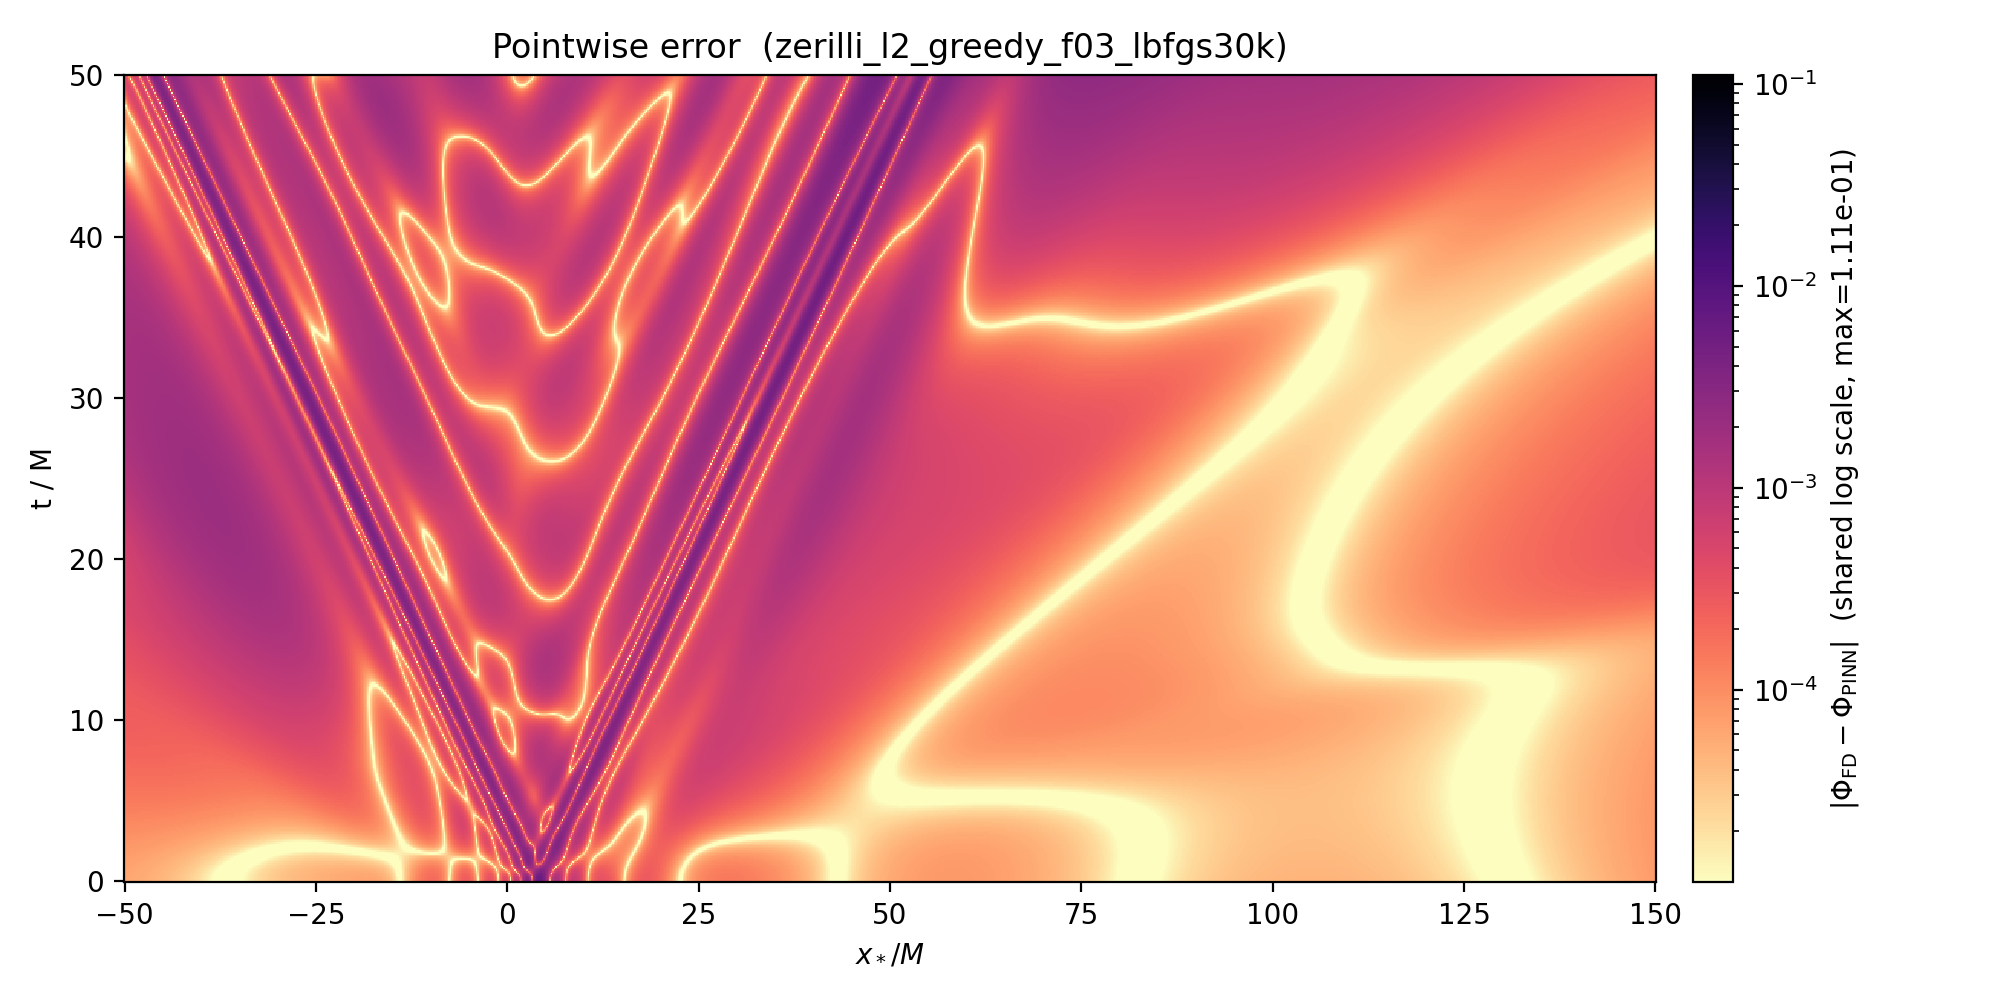
\includegraphics[width=\linewidth,height=0.70\textheight,keepaspectratio]{../outputs/pinn/zerilli_l2_greedy_f03_lbfgs30k/error_heatmap.png}
      \\[3pt]{\scriptsize Pointwise error $|\Phi_{\pinn{}}-\Phi_{\fd{}}|$ over the
      full $(x,t)$ domain.}
    \end{column}
    \begin{column}{0.48\textwidth}
      \centering
      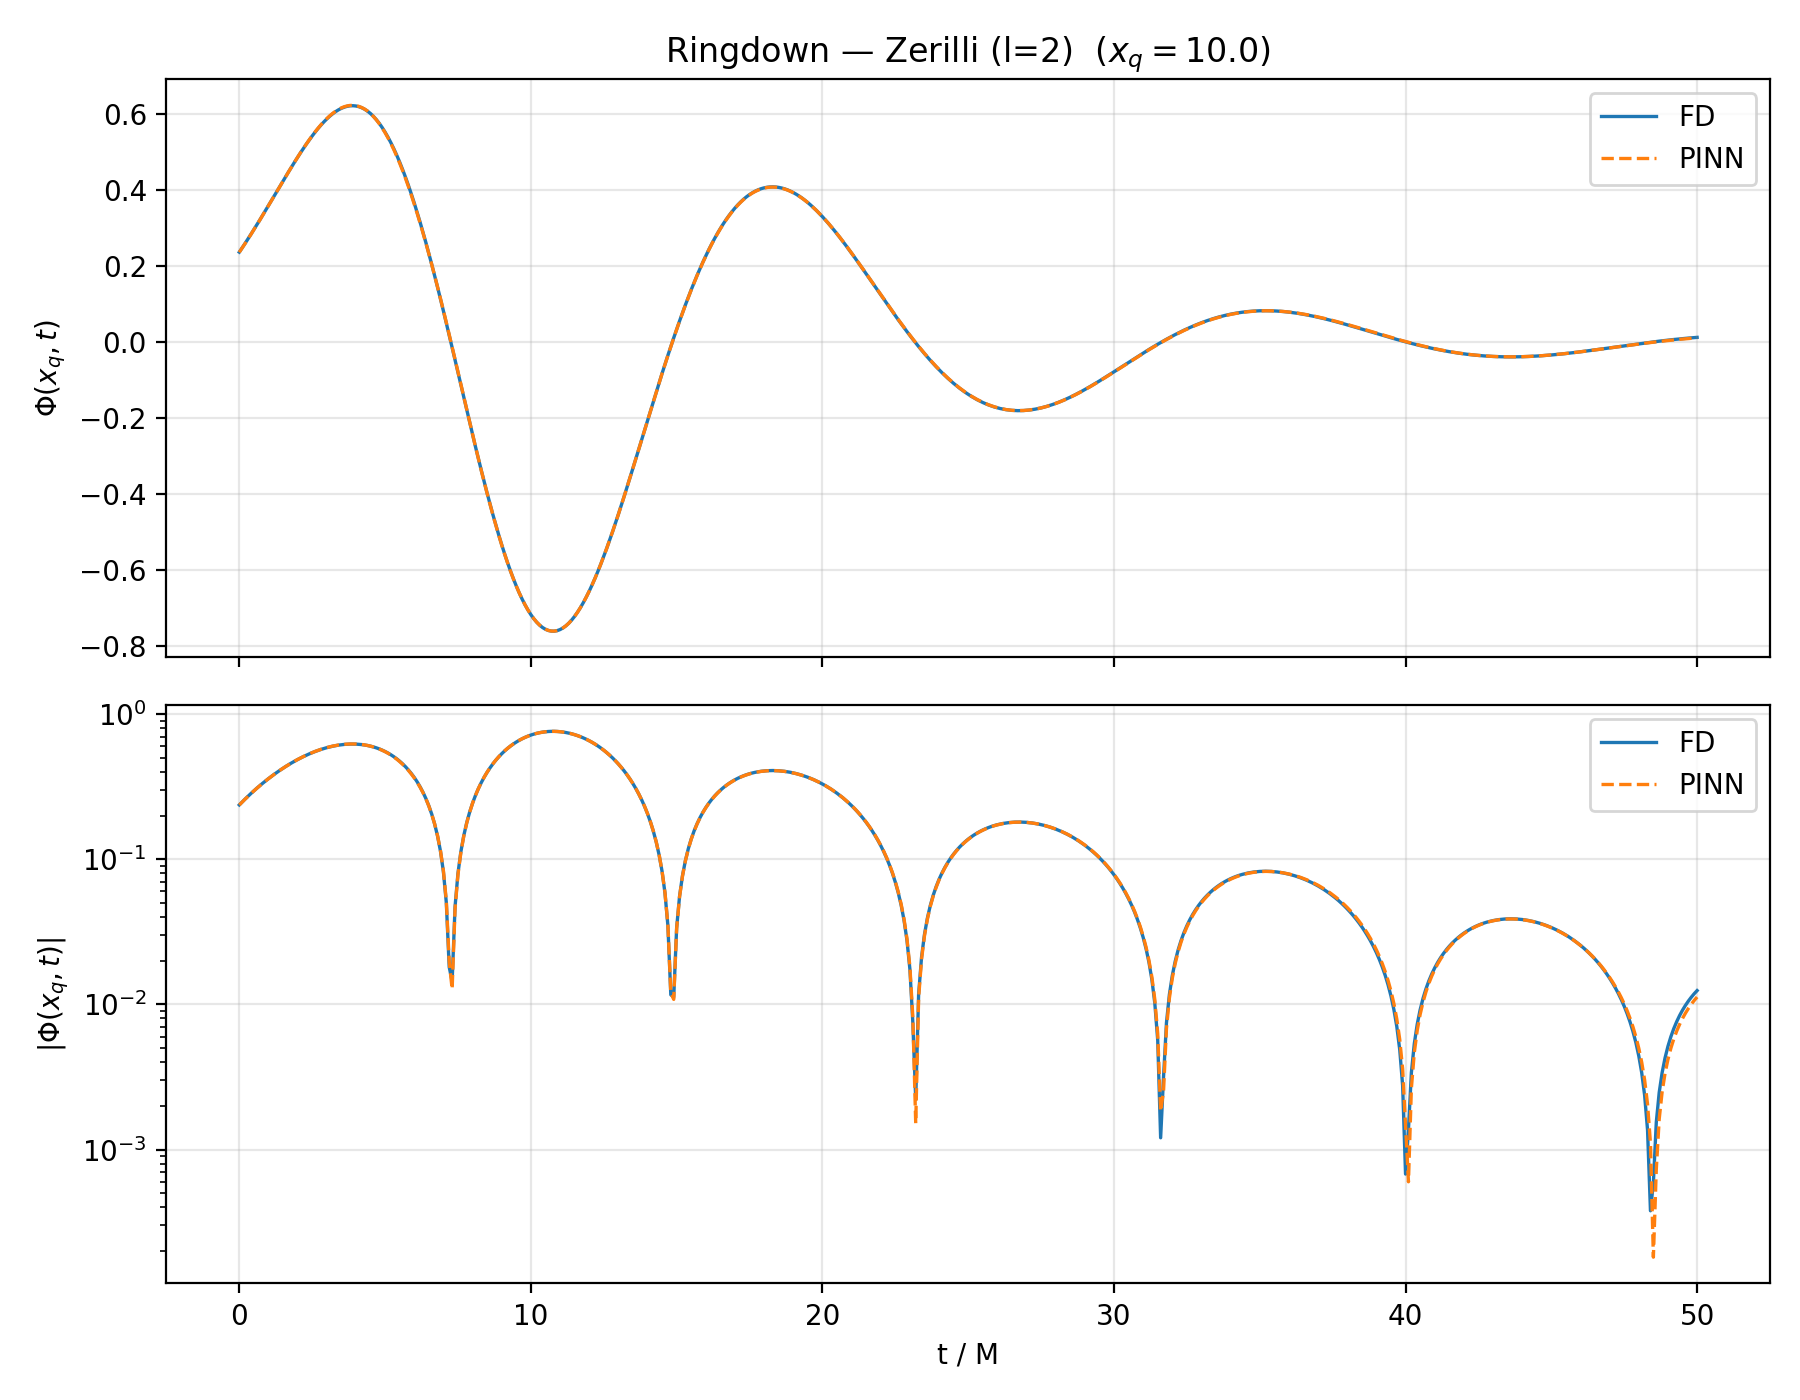
\includegraphics[width=\linewidth,height=0.70\textheight,keepaspectratio]{../outputs/pinn/zerilli_l2_greedy_f03_lbfgs30k/ringdown_overlay.png}
      \\[3pt]{\scriptsize Ringdown overlay at $x_{q}\!=\!10\,M$: PINN (solid)
      vs.\ FD (dashed). Greedy resampling, $f\!=\!0.3$, $+$ L-BFGS 30k.}
    \end{column}
  \end{columns}
\end{frame}

\begin{frame}{Forward PINN --- waveform snapshots and pointwise error}
  \begin{columns}[T]
    \begin{column}{0.50\textwidth}
      \centering
      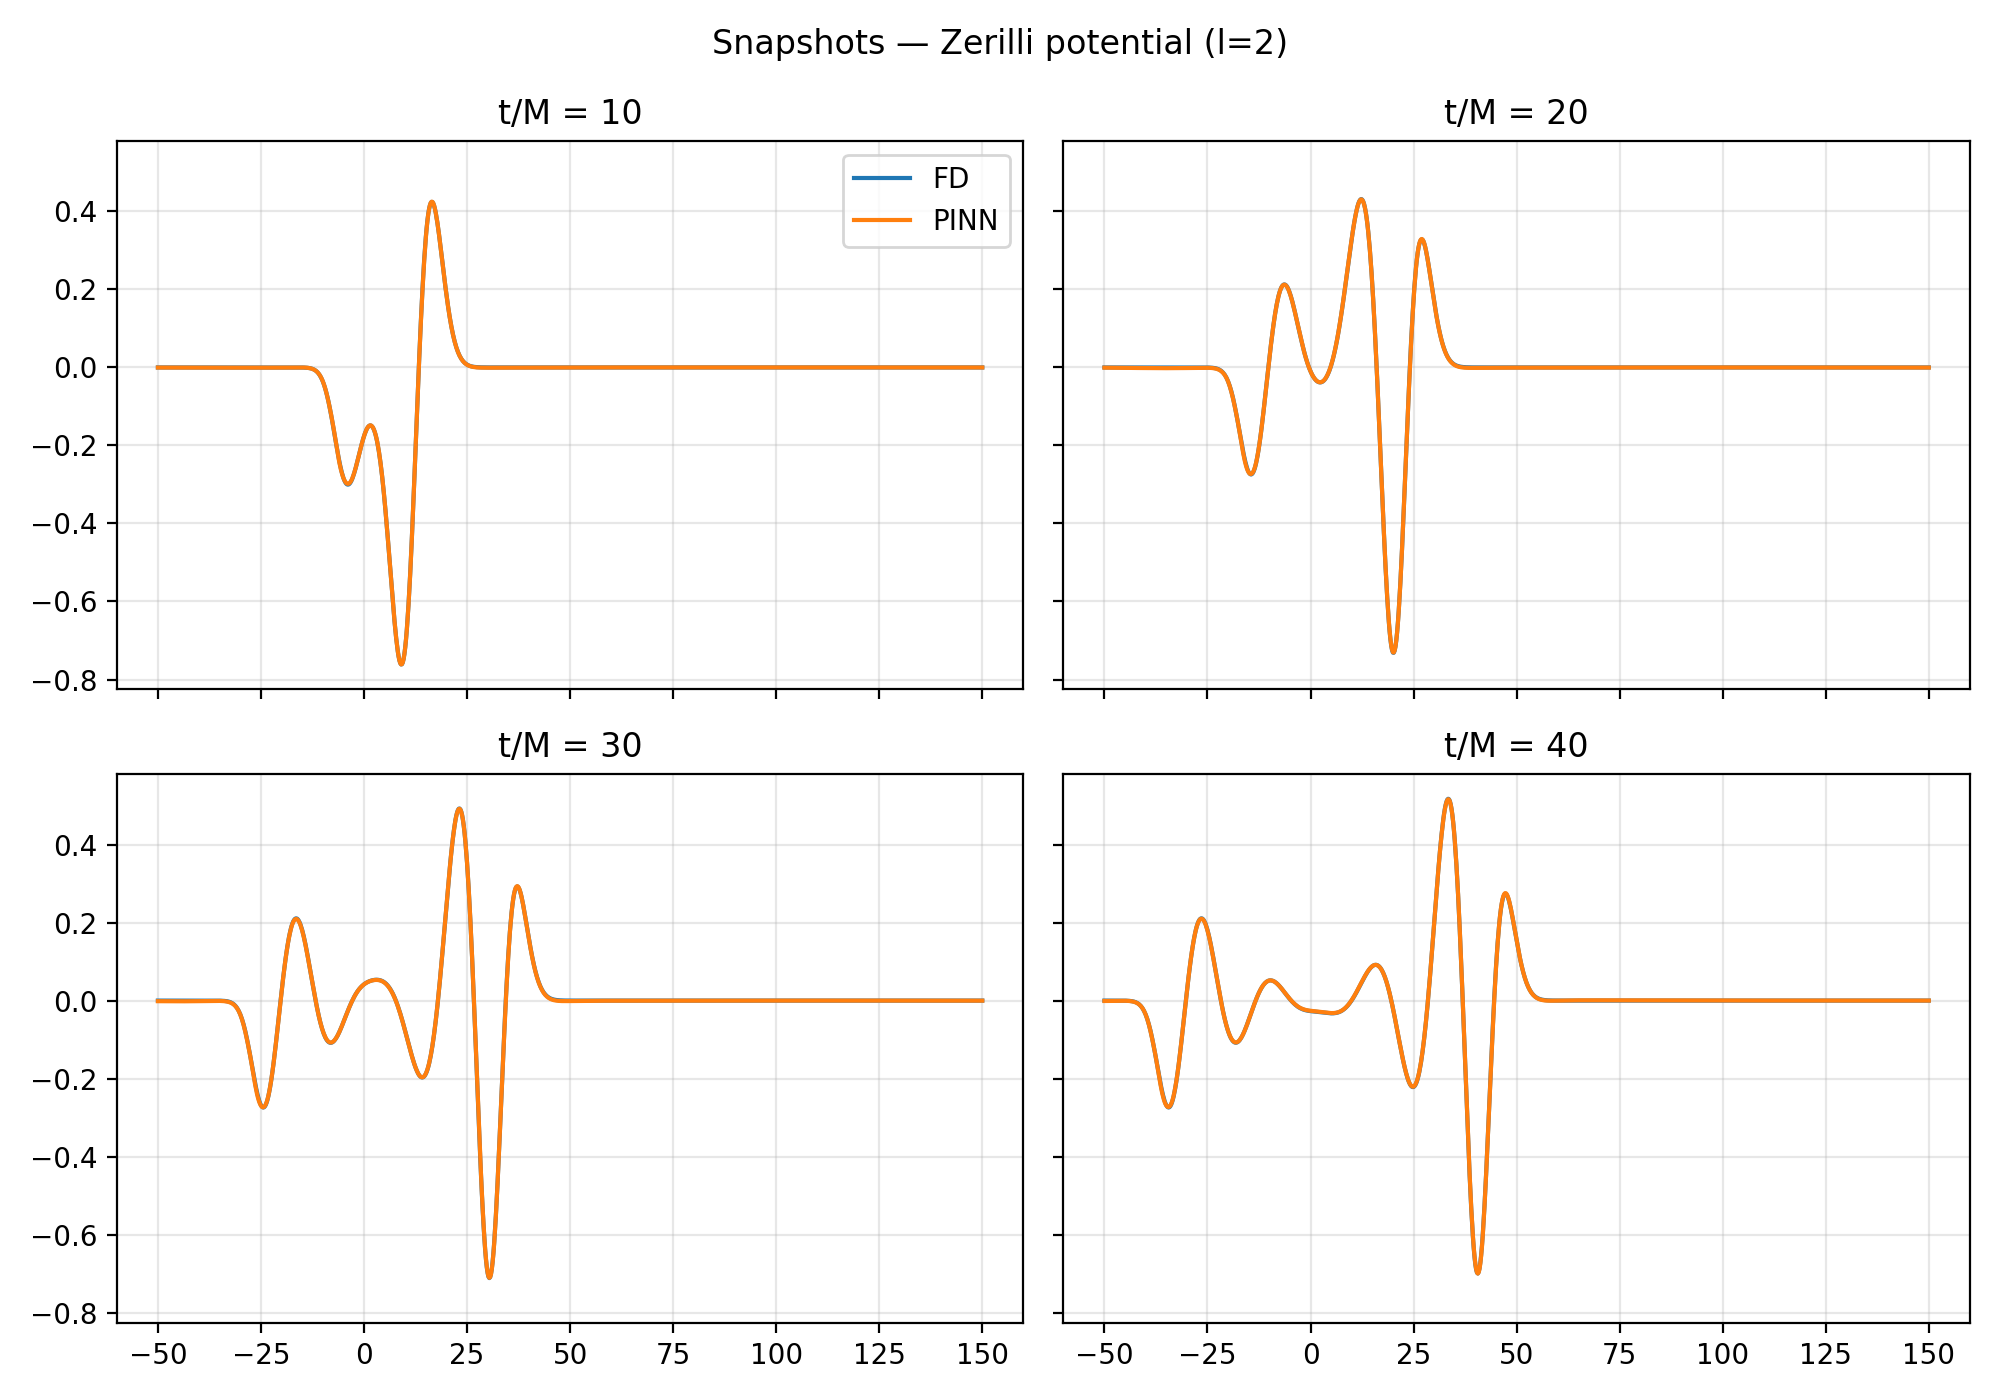
\includegraphics[width=\textwidth,height=0.72\textheight,keepaspectratio]{../outputs/pinn/zerilli_l2_greedy_f03_lbfgs30k/snapshots.png}
      \\[2pt]{\scriptsize $\Phi_{\pinn{}}$ (solid) vs.\ $\Phi_{\fd{}}$ (dashed) at
      $t/M\!\in\!\{10,20,30,40\}$.}
    \end{column}
    \begin{column}{0.48\textwidth}
      \centering
      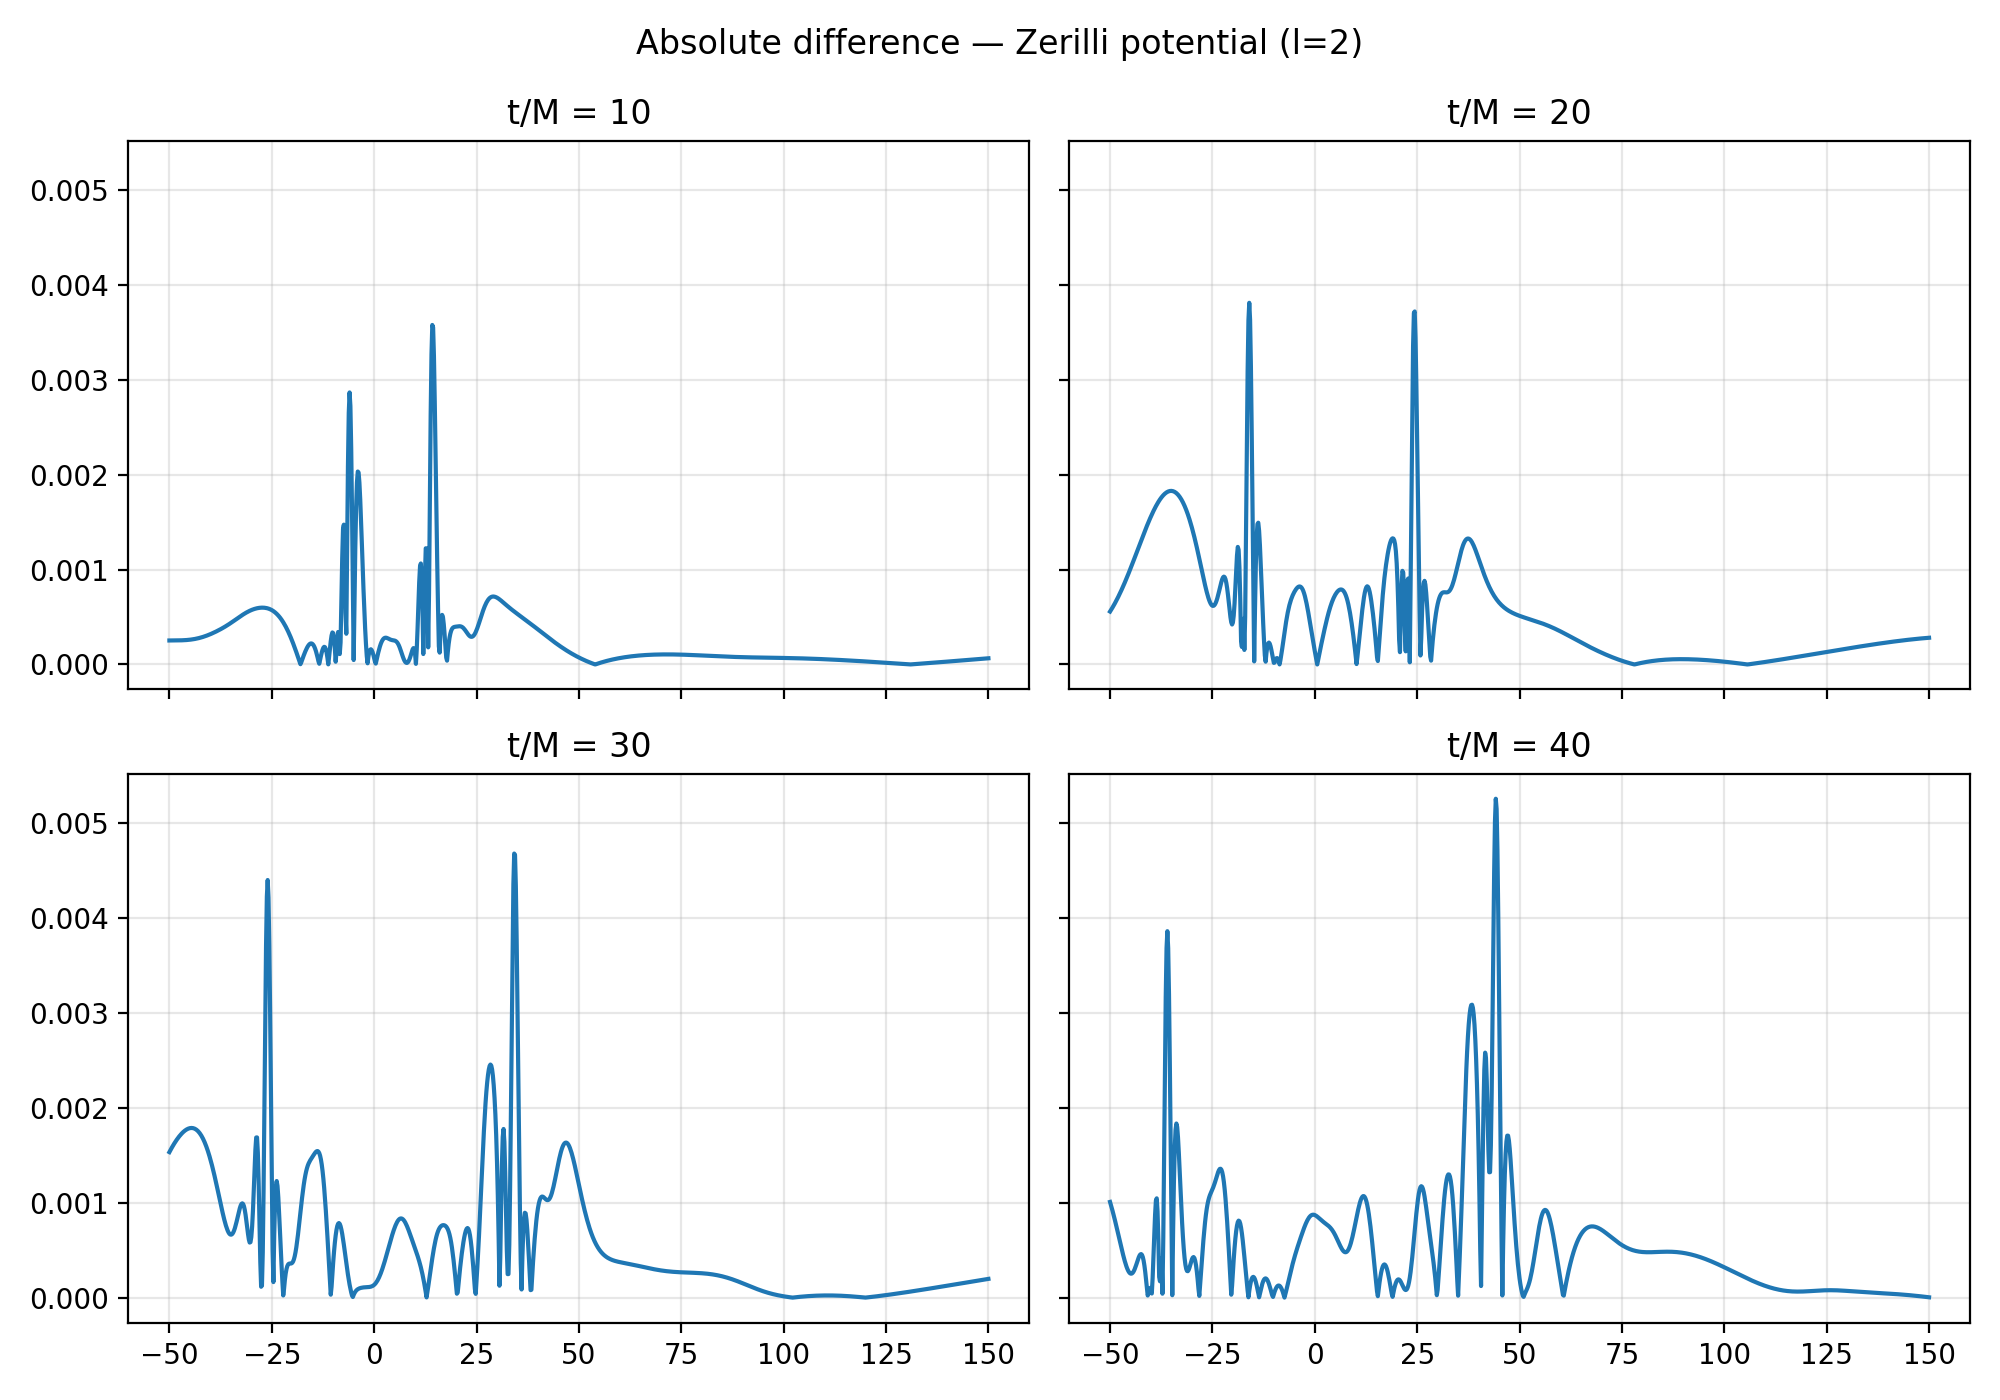
\includegraphics[width=\textwidth,height=0.72\textheight,keepaspectratio]{../outputs/pinn/zerilli_l2_greedy_f03_lbfgs30k/abs_diff_snapshots.png}
      \\[2pt]{\scriptsize Pointwise $|\Phi_{\pinn{}}-\Phi_{\fd{}}|$ at the same
      times: residual $\lesssim\!5\!\times\!10^{-3}$ near the barrier, $\lesssim\!10^{-3}$ far away.}
    \end{column}
  \end{columns}
\end{frame}

\begin{frame}{Forward PINN --- zoomed late-time waveform and error}
  \begin{columns}[T]
    \begin{column}{0.50\textwidth}
      \centering
      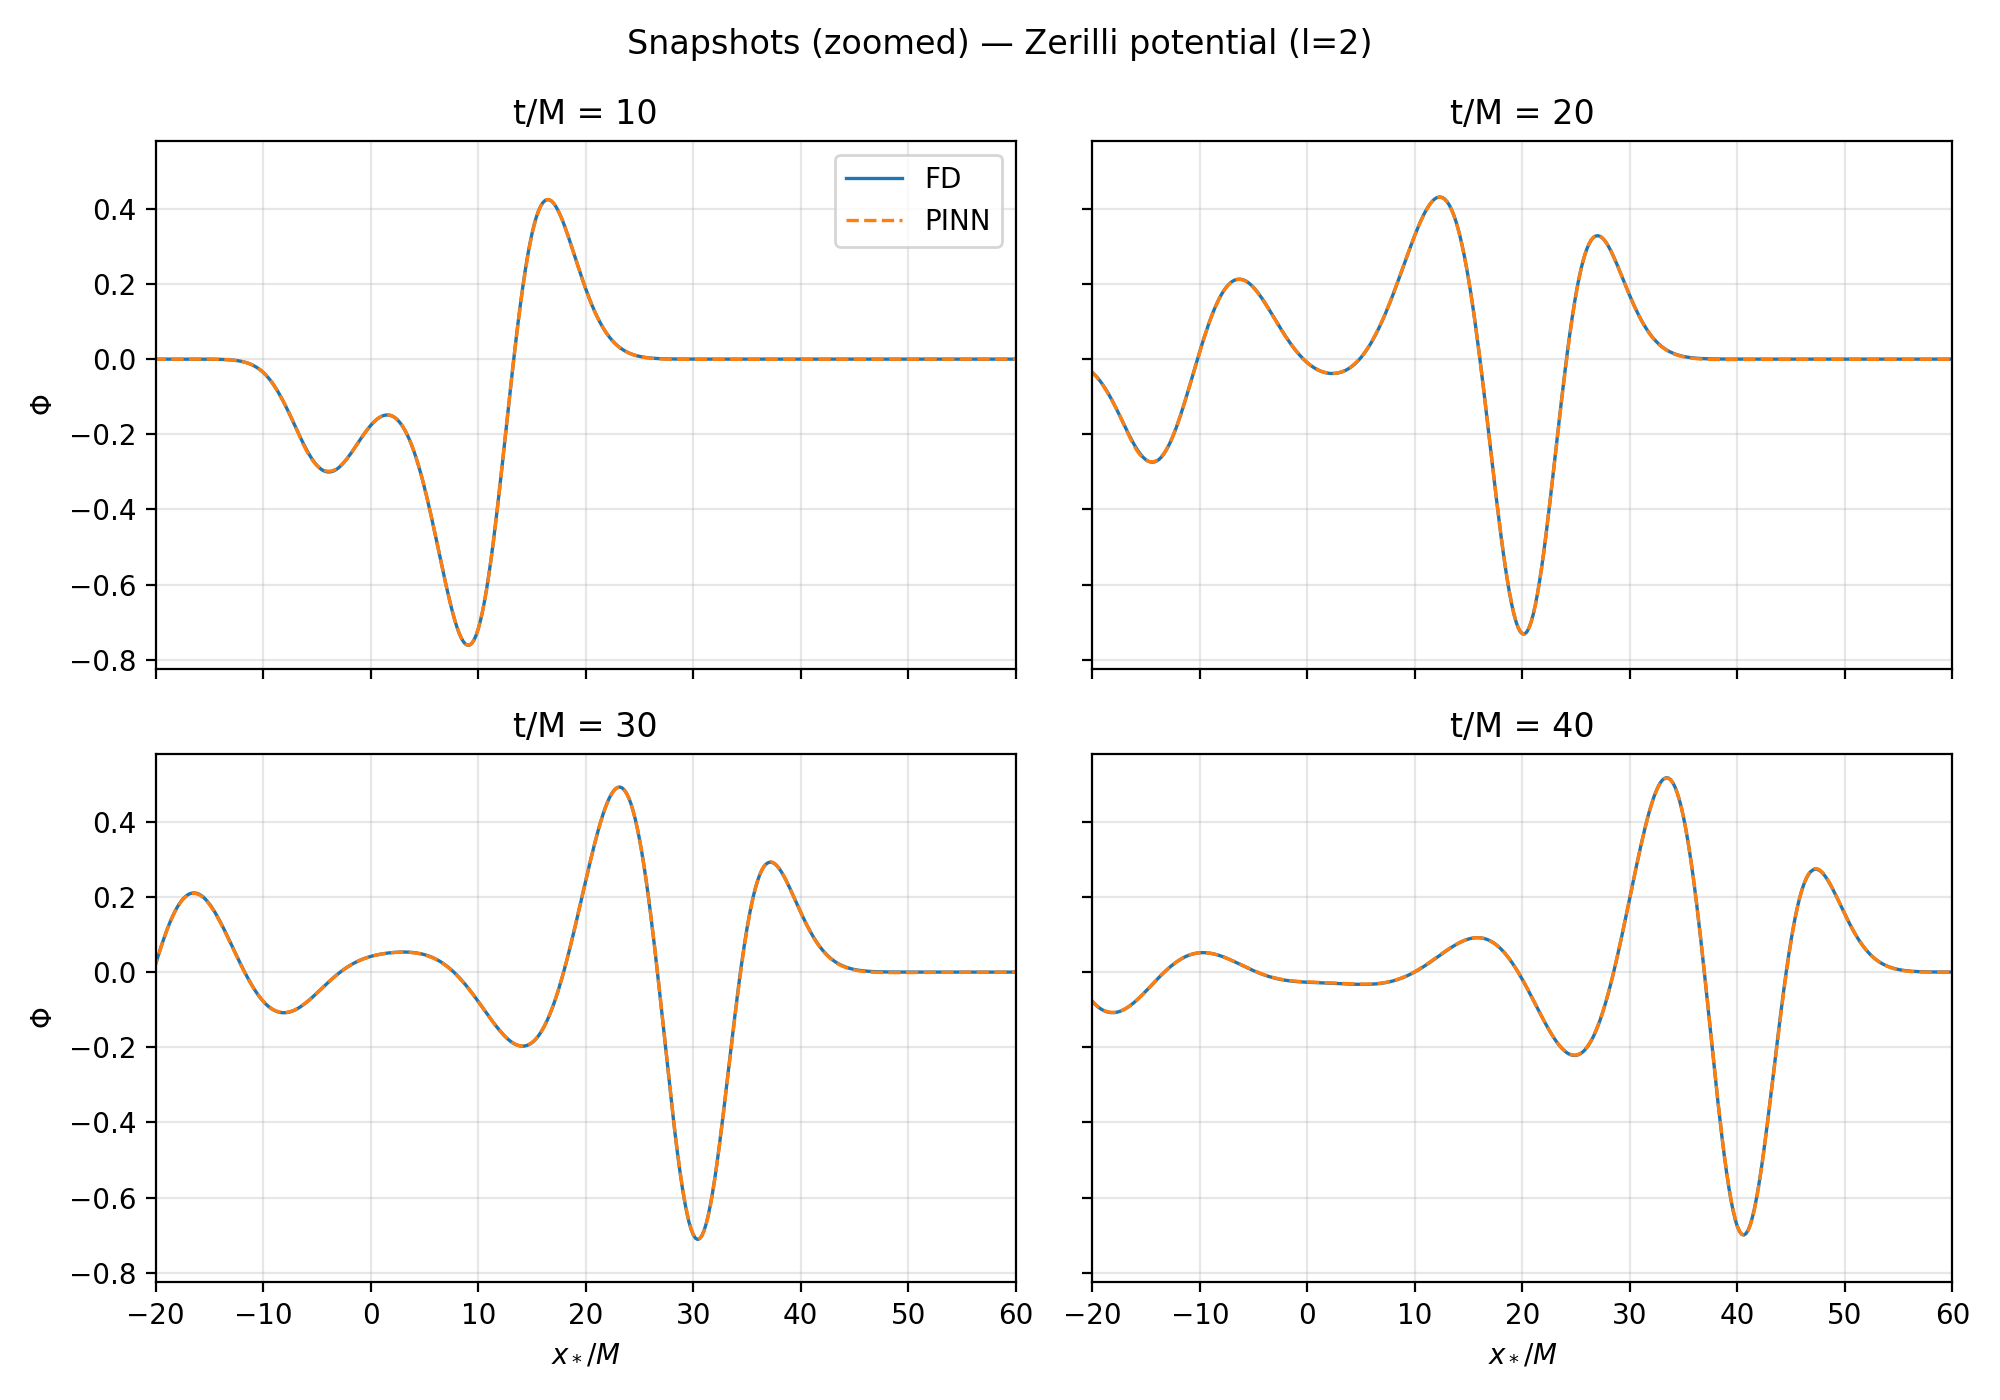
\includegraphics[width=\textwidth,height=0.72\textheight,keepaspectratio]{../outputs/pinn/zerilli_l2_greedy_f03_lbfgs30k/snapshots_zoomed.png}
      \\[2pt]{\scriptsize Zoomed snapshots near the potential barrier; the
      PINN tracks both phase and decay envelope of the FD ground truth.}
    \end{column}
    \begin{column}{0.48\textwidth}
      \centering
      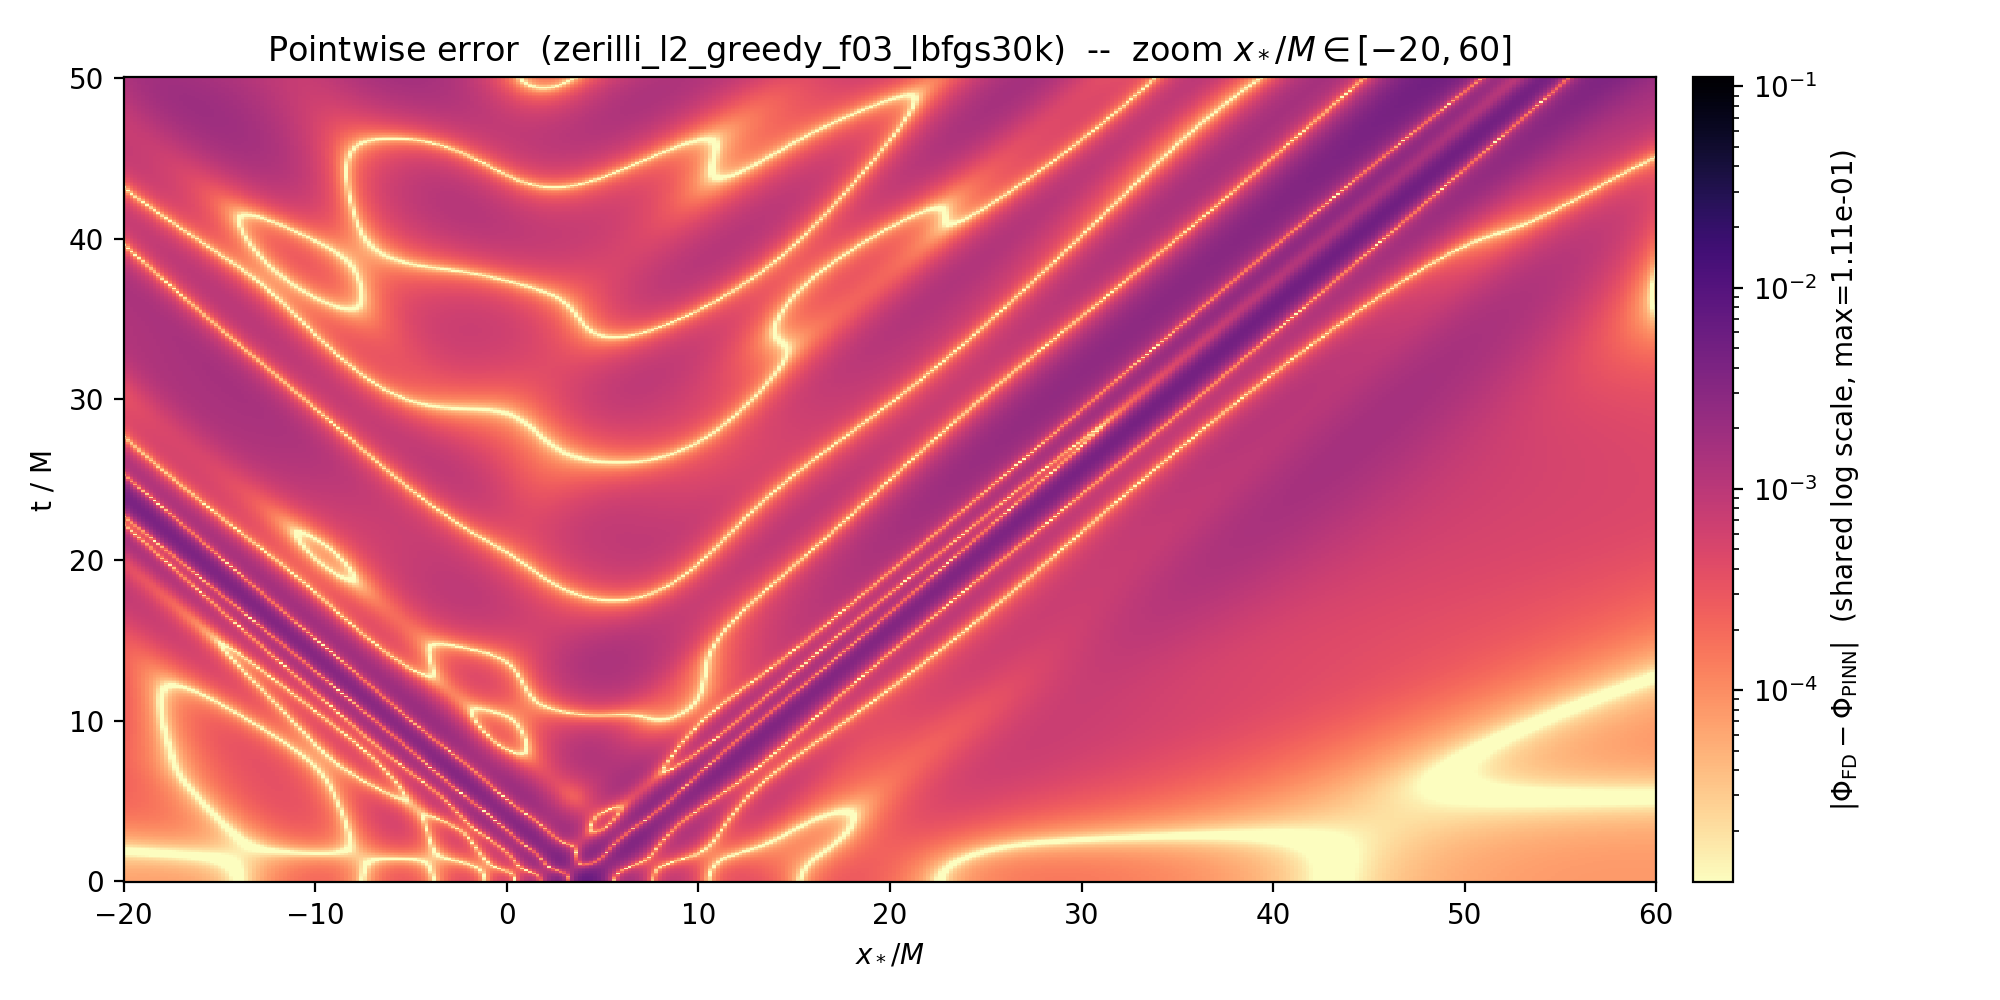
\includegraphics[width=\textwidth,height=0.72\textheight,keepaspectratio]{../outputs/pinn/zerilli_l2_greedy_f03_lbfgs30k/error_heatmap_zoomed.png}
      \\[2pt]{\scriptsize Zoomed pointwise error: residual concentrated on
      the prompt burst $t\!\lesssim\!15M$, near-uniform during the ringdown.}
    \end{column}
  \end{columns}
\end{frame}

\begin{frame}{Forward PINN --- best result: \qnm{} accuracy}
  \centering
  \renewcommand{\arraystretch}{1.25}
  \begin{tabular}{@{}lccc@{}}
    \toprule
    \textbf{Quantity} & \textbf{Our value} & \textbf{Leaver reference} & \textbf{Error} \\
    \midrule
    RMSD vs.\ \fd{}                  & $8.17\!\times\!10^{-4}$ & ---     & --- \\
    $\omega$  (M4 plateau)           & $0.37359$               & $0.37367$ & \textcolor{darkgreen}{\textbf{0.029\%}} \\
    $\tau$    (M2, window $[10,50]M$) & $11.46$                 & $11.241$  & $1.99\%$ \\
    \bottomrule
  \end{tabular}
  \vspace{6mm}

  \fbox{\parbox{0.85\textwidth}{\centering
    Patel et al.\ 2024 report $\sim\!1\%$ accuracy on $\omega$.\\
    \textbf{We reach $0.03\%$ --- a $\sim\!30\times$ improvement.}}}
\end{frame}


% ══════════════════════════════════════════════════════════════════
\section{3. Inverse PINN}
% ══════════════════════════════════════════════════════════════════

\begin{frame}{Inverse PINN --- problem statement}
  \textbf{Forward problem:} given $M$ (hence $V(r;M)$), solve for the field
  $\Phi(x,t)$.\\
  \textbf{Inverse problem:} given an observed waveform $\Phi_{\!\fd{}}(x,t)$,
  recover the underlying physical parameters
  $\bigl(M,\,\omega,\,\tau\bigr)$.
  \bigskip

  We minimise a sum of \textbf{nine} weighted mean-squared-error terms:
  the seven forward losses (with $V$ now evaluated at the \emph{learned}
  mass $M$) plus two new data-driven terms,
  \[
    \mathcal{L}_{\text{inv}}
    \;=\;
    \underbrace{\textcolor{darkred}{\mathcal{L}_{\text{PDE}+\text{gPINN}}(M)}}_{\text{Zerilli residual at learned }M}
    \;+\;
    \underbrace{\textcolor{darkgreen}{\mathcal{L}_{\text{IC}+\text{BC}}}}_{\text{geometry}}
    \;+\;
    \underbrace{\textcolor{blue}{\lambda_{\text{data}}\,\mathcal{L}_{\text{data}}}}_{\text{noisy waveform fit}}
    \;+\;
    \underbrace{\textcolor{purple}{\lambda_{\text{ring}}\,\mathcal{L}_{\text{ring}}}}_{\text{ringdown-template fit}}
  \]
  \bigskip

  Five physical scalars
  $(M,\,\omega,\,\tau,\,A_{\mathrm{ring}},\,\phi)$
  are appended to the optimiser's parameter list and trained
  \emph{jointly} with the network weights $\boldsymbol{\theta}$.
  The next slide writes the two new sums explicitly.
\end{frame}

\begin{frame}{Inverse PINN loss --- data and ringdown terms}
  \footnotesize
  \textcolor{blue}{\textbf{Data loss}} on
  $N_{\mathrm{obs}}\!=\!500$ randomly drawn observation points
  $\{(x_{j},t_{j})\}_{j=1}^{N_{\mathrm{obs}}}$ with FD reference values
  $\Phi_{\!\fd{}}(x_{j},t_{j})$:
  \[
    \textcolor{blue}{\mathcal{L}_{\mathrm{data}}}
      \;=\; \frac{1}{N_{\mathrm{obs}}}\sum_{j=1}^{N_{\mathrm{obs}}}
            \bigl[\,\Phi_{\theta}(x_{j},t_{j})
                  -\Phi_{\!\fd{}}(x_{j},t_{j})\,\bigr]^{2}.
  \]
  \medskip
  \textcolor{purple}{\textbf{Ringdown-template loss}} at the observer
  column $x_{q}\!=\!10\,M$, on $N_{\mathrm{ring}}$ time samples
  $\{t_{k}\}_{k=1}^{N_{\mathrm{ring}}}$ in the late-time window
  $t_{k}\in[\,t_{\mathrm{ring}}^{\min},\,t_{\max}\,]$:
  \[
    \textcolor{purple}{\mathcal{L}_{\mathrm{ring}}}
      \;=\; \frac{1}{N_{\mathrm{ring}}}\sum_{k=1}^{N_{\mathrm{ring}}}
            \Bigl[\,\Phi_{\theta}(x_{q},t_{k})
                  \;-\;
                  A_{\mathrm{ring}}\,e^{-t_{k}/\tau}\cos(\omega t_{k}+\phi)\,\Bigr]^{2}.
  \]
  \medskip
  Through this sum, the four template scalars
  $(\omega,\tau,A_{\mathrm{ring}},\phi)$ receive gradients directly from
  the late-time portion of $\Phi_{\theta}$, while $M$ receives gradients
  through $\mathcal{L}_{\mathrm{PDE}+\mathrm{gPINN}}(M)$ via $V(r;M)$.
\end{frame}

\begin{frame}{Inverse PINN --- training setup}
  \begin{itemize}
    \item \textbf{Network.} Identical $[\,2,80,40,20,10,1\,]$ $\tanh$ MLP
          and output transform as the forward PINN.
    \item \textbf{Learnable physical parameters} (initial values):
          $M_{\mathrm{init}}\!=\!1.20$ (twenty per cent above the truth),
          $\omega_{\mathrm{init}}\!=\!0.30$,
          $\tau_{\mathrm{init}}\!=\!8.00$,
          $A_{\mathrm{ring,\,init}}$ and $\phi_{\mathrm{init}}$ from a
          short pre-fit on the FD waveform.
    \item \textbf{Loss weights} for the two new terms:
          $\lambda_{\mathrm{data}}\!=\!1$,
          $\lambda_{\mathrm{ring}}\!=\!100$. Forward weights unchanged.
    \item \textbf{Optimiser.} Adam ($10{,}000$ steps) followed by L-BFGS
          ($30{,}000$ steps); the five physical scalars and the network
          weights are updated together in every step.
    \item \textbf{Variant D combo:}
          $t_{\mathrm{ring}}^{\min}\!=\!18\,M$,
          $N_{\mathrm{ring}}\!=\!1000$, late-time window only ---
          our best configuration.
  \end{itemize}
\end{frame}

\begin{frame}{Inverse PINN --- our architecture}
  \centering
  \resizebox{0.95\textwidth}{!}{%
  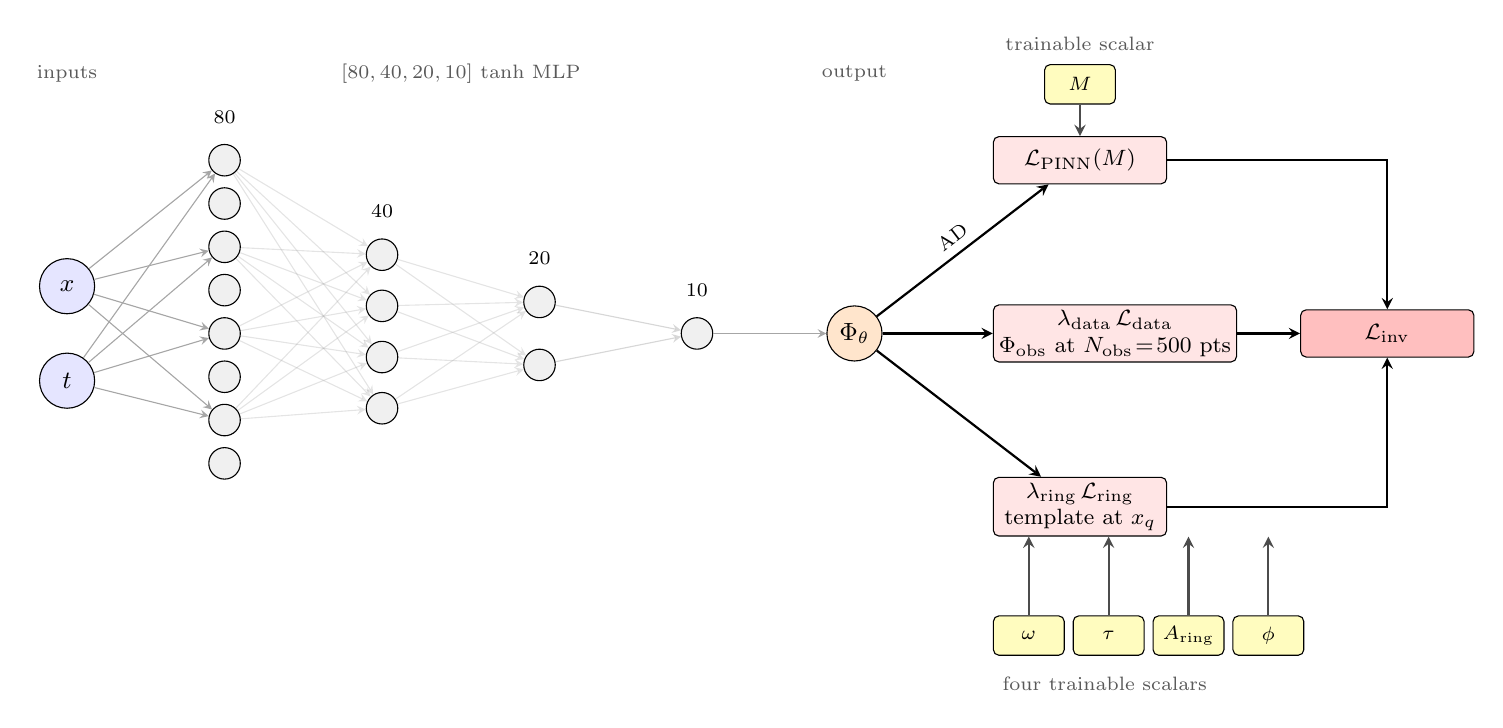
\begin{tikzpicture}[
    node distance=10mm and 12mm,
    every node/.style={font=\small},
    inp/.style={circle, draw, fill=blue!10, minimum size=7mm, inner sep=0pt},
    hid/.style={circle, draw, fill=gray!12, minimum size=4mm, inner sep=0pt},
    outn/.style={circle, draw, fill=orange!20, minimum size=7mm, inner sep=0pt},
    var/.style={rectangle, draw, fill=yellow!25, rounded corners=2pt,
                minimum height=5mm, minimum width=9mm, inner sep=2pt,
                font=\scriptsize, align=center},
    loss/.style={rectangle, draw, fill=red!10, rounded corners=2pt,
                 minimum height=6mm, minimum width=22mm, inner sep=2pt,
                 align=center, font=\footnotesize},
    arr/.style={->, >=stealth, thin, gray!70},
  ]
    \node[inp] (x) at (0, 0) {$x$};
    \node[inp] (t) at (0, -1.2) {$t$};
    \def\xL{2.0}\def\xLii{4.0}\def\xLiii{6.0}\def\xLiv{8.0}
    \foreach \k/\y in {1/1.6, 2/1.05, 3/0.5, 4/-0.05, 5/-0.6, 6/-1.15, 7/-1.7, 8/-2.25}{
      \node[hid] (a\k) at (\xL, \y) {};}
    \foreach \k/\y in {1/0.4, 2/-0.25, 3/-0.9, 4/-1.55}{
      \node[hid] (b\k) at (\xLii, \y) {};}
    \foreach \k/\y in {1/-0.2, 2/-1.0}{
      \node[hid] (c\k) at (\xLiii, \y) {};}
    \node[hid] (d1) at (\xLiv, -0.6) {};
    \node[font=\scriptsize] at (\xL, 2.15) {$80$};
    \node[font=\scriptsize] at (\xLii, 0.95) {$40$};
    \node[font=\scriptsize] at (\xLiii, 0.35) {$20$};
    \node[font=\scriptsize] at (\xLiv, -0.05) {$10$};
    \node[outn] (phi) at (10.0, -0.6) {$\Phi_\theta$};
    \foreach \src in {x, t}\foreach \dst in {a1, a3, a5, a7}\draw[arr] (\src) -- (\dst);
    \foreach \a in {1,3,5,7}\foreach \b in {1,2,3,4}\draw[arr, opacity=0.30] (a\a) -- (b\b);
    \foreach \a in {1,2,3,4}\foreach \b in {1,2}\draw[arr, opacity=0.30] (b\a) -- (c\b);
    \foreach \a in {1,2}\draw[arr, opacity=0.45] (c\a) -- (d1);
    \draw[arr] (d1) -- (phi);
    \node[loss, right=14mm of phi, yshift=22mm] (lpinn)
      {$\mathcal{L}_{\mathrm{PINN}}(M)$};
    \node[loss, right=14mm of phi] (ldata)
      {$\lambda_{\mathrm{data}}\,\mathcal{L}_{\mathrm{data}}$\\$\Phi_{\mathrm{obs}}$ at $N_{\mathrm{obs}}\!=\!500$ pts};
    \node[loss, right=14mm of phi, yshift=-22mm] (lring)
      {$\lambda_{\mathrm{ring}}\,\mathcal{L}_{\mathrm{ring}}$\\template at $x_q$};
    \draw[arr, thick, black] (phi) -- (lpinn) node[midway, above, font=\scriptsize, sloped] {AD};
    \draw[arr, thick, black] (phi) -- (ldata);
    \draw[arr, thick, black] (phi) -- (lring);
    \node[var, above=4mm of lpinn] (vM) {$M$};
    \node[font=\scriptsize, gray!70!black, above=0.5mm of vM] {trainable scalar};
    \draw[arr, thick, black!70] (vM) -- (lpinn);
    \node[var, below=10mm of lring.south west, anchor=north west] (vom) {$\omega$};
    \node[var, right=1mm of vom]   (vtau)  {$\tau$};
    \node[var, right=1mm of vtau]  (vA)    {$A_{\mathrm{ring}}$};
    \node[var, right=1mm of vA]    (vphi0) {$\phi$};
    \node[font=\scriptsize, gray!70!black, below=1.5mm of vom.south west, anchor=north west]
      {four trainable scalars};
    \draw[arr, thick, black!70] (vom.north)   -- (vom.north   |- lring.south);
    \draw[arr, thick, black!70] (vtau.north)  -- (vtau.north  |- lring.south);
    \draw[arr, thick, black!70] (vA.north)    -- (vA.north    |- lring.south);
    \draw[arr, thick, black!70] (vphi0.north) -- (vphi0.north |- lring.south);
    \node[loss, fill=red!25, right=8mm of ldata] (ltot)
      {$\mathcal{L}_{\mathrm{inv}}$};
    \draw[arr, thick, black] (lpinn) -| (ltot);
    \draw[arr, thick, black] (ldata) -- (ltot);
    \draw[arr, thick, black] (lring) -| (ltot);
    \node[font=\scriptsize, gray!70!black] at (0.0, 2.7) {inputs};
    \node[font=\scriptsize, gray!70!black] at (5.0, 2.7) {$[80,40,20,10]$ tanh MLP};
    \node[font=\scriptsize, gray!70!black] at (10.0, 2.7) {output};
  \end{tikzpicture}}
  \\[6pt]
  \begin{minipage}{0.92\textwidth}
    \centering\scriptsize
    Same $[80,40,20,10]$ $\tanh$ MLP as the forward PINN, with five physical
    scalars $(M,\omega,\tau,A_{\mathrm{ring}},\phi)$ (yellow) appended to the
    optimiser's parameter list. $M$ enters the PDE residual through $V(r;M)$;
    $(\omega,\tau,A_{\mathrm{ring}},\phi)$ enter $\mathcal{L}_{\mathrm{ring}}$
    at the observer column $x_{q}\!=\!10\,M$.
  \end{minipage}
\end{frame}

\begin{frame}{Inverse PINN --- best result (variant D ``combo''): waveform}
  \begin{columns}[T]
    \begin{column}{0.50\textwidth}
      \centering
      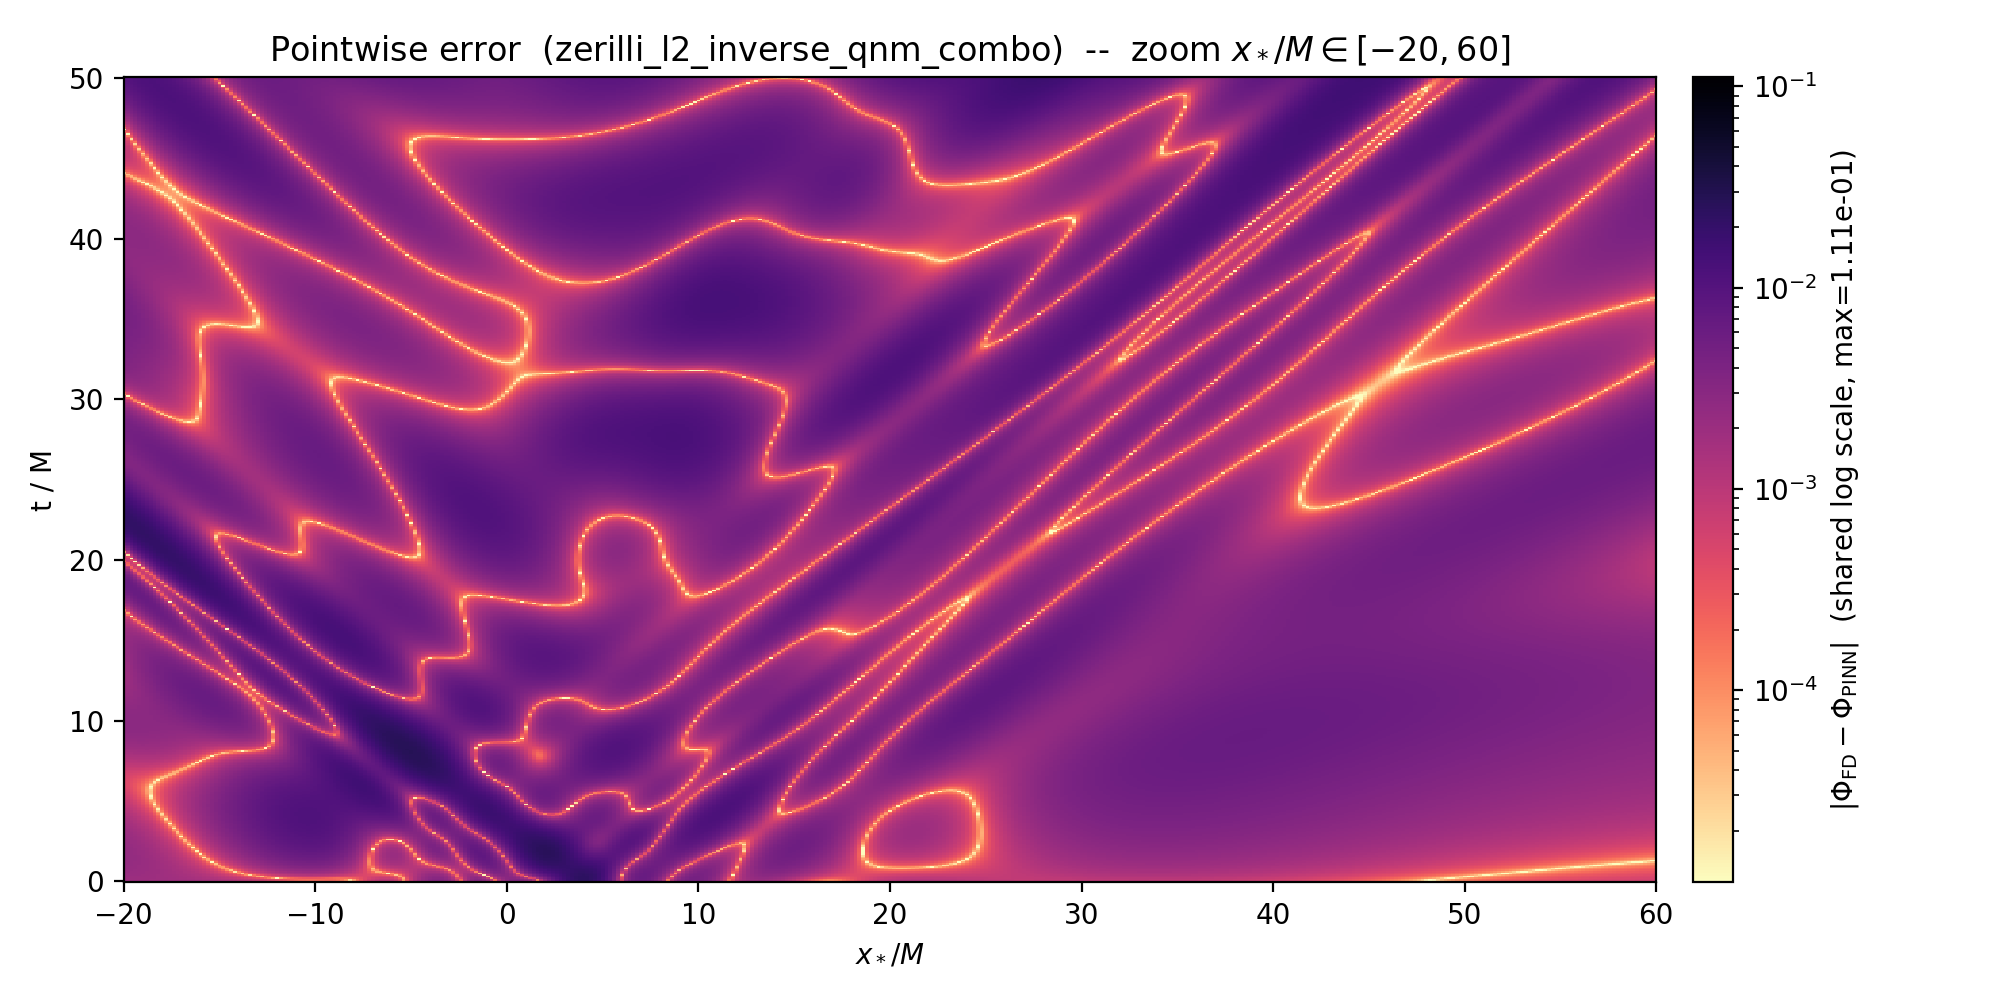
\includegraphics[width=\textwidth]{../outputs/pinn/zerilli_l2_inverse_qnm_combo/error_heatmap_zoomed.png}
      \\{\scriptsize $|\Phi_\theta - \Phi_{\fd{}}|$ on the zoomed late-time region.}
    \end{column}
    \begin{column}{0.48\textwidth}
      \centering
      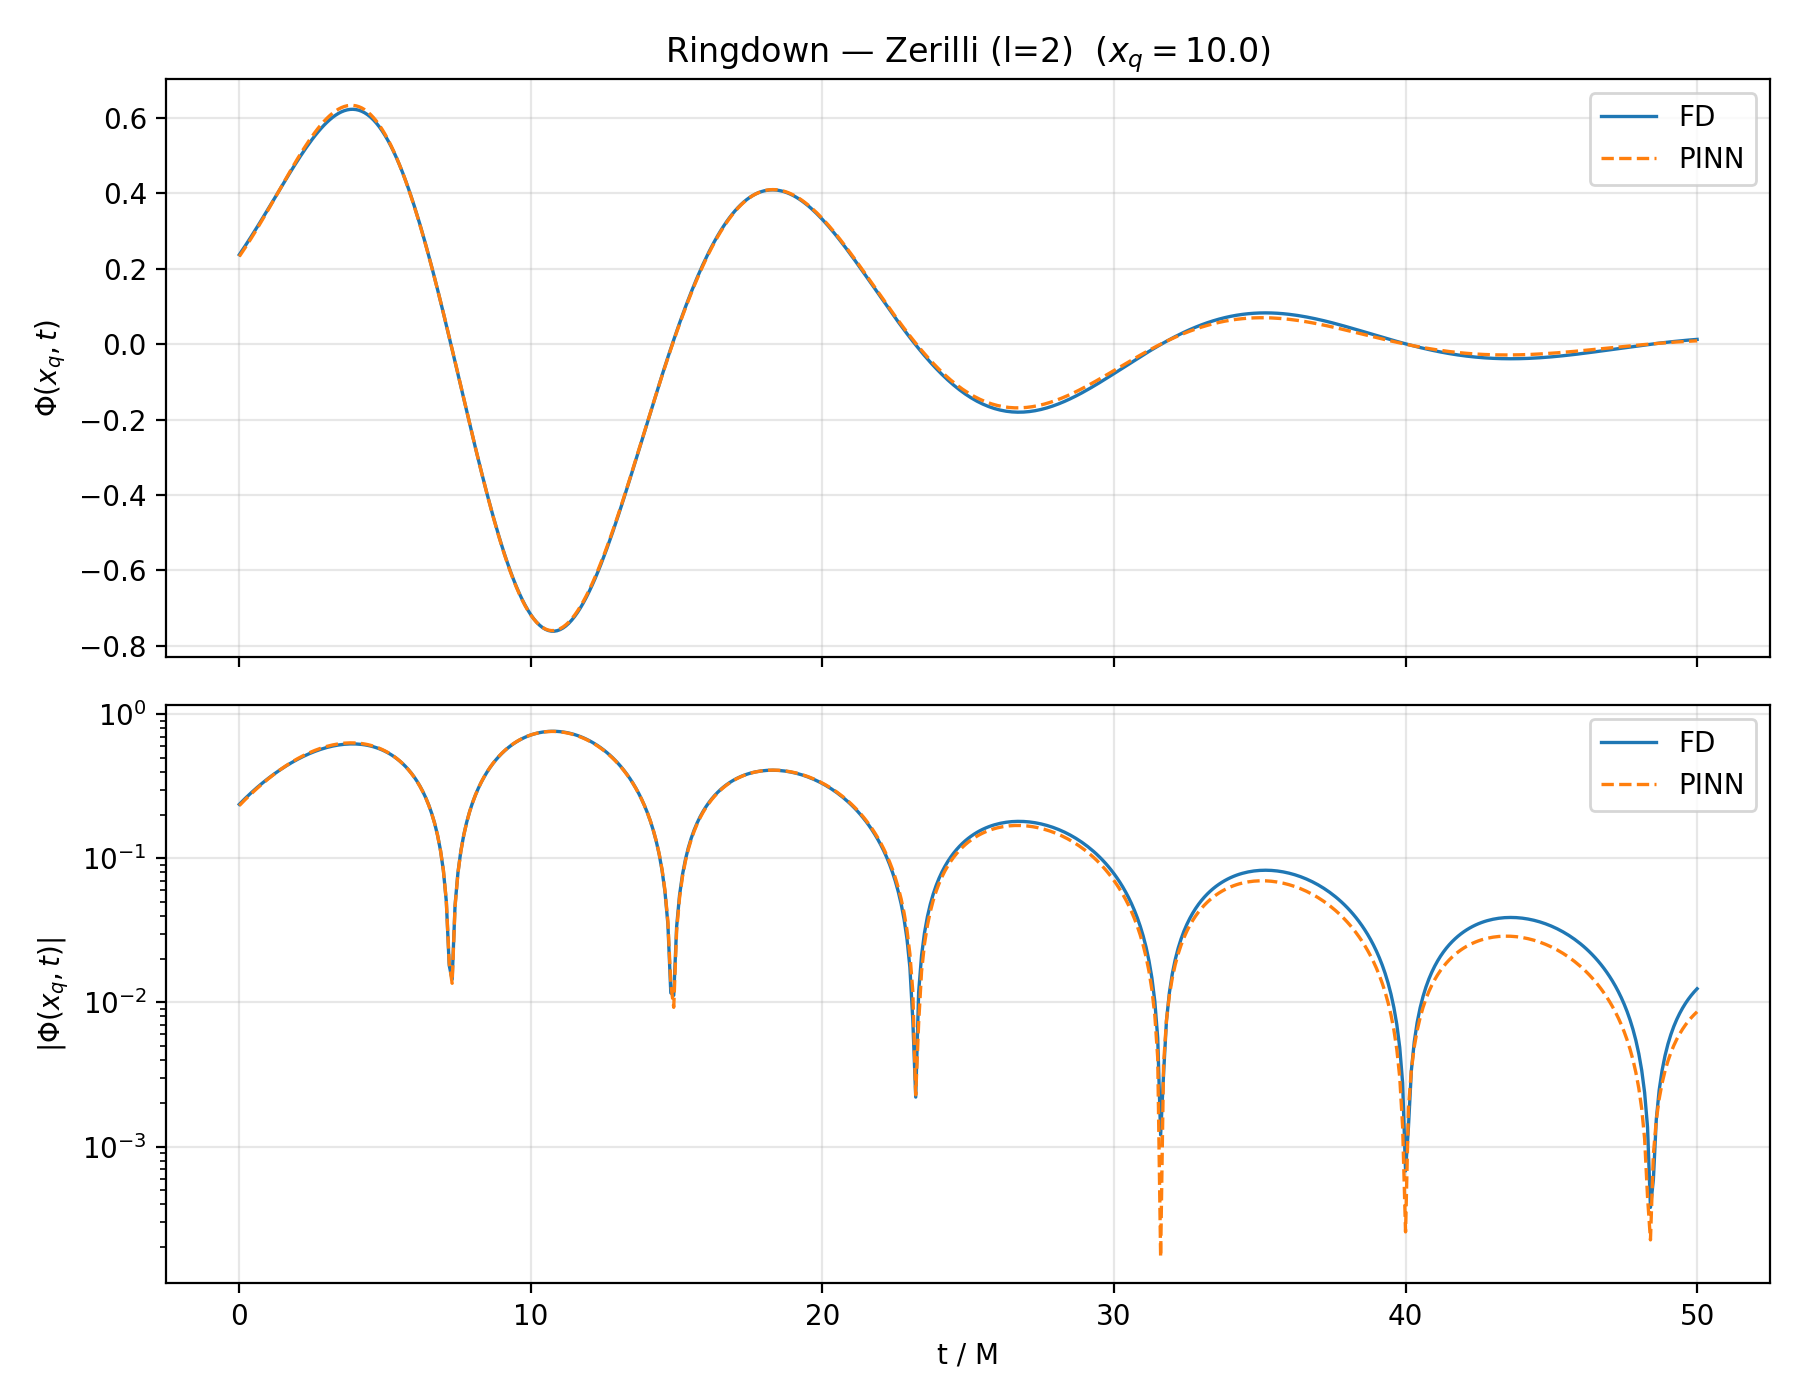
\includegraphics[width=\textwidth]{../outputs/pinn/zerilli_l2_inverse_qnm_combo/ringdown_overlay.png}
      \\{\scriptsize PINN ringdown at $x_{q}\!=\!10\,M$ vs.\ \fd{} ground truth.}
    \end{column}
  \end{columns}
\end{frame}

\begin{frame}{Inverse PINN --- waveform snapshots and pointwise error}
  \begin{columns}[T]
    \begin{column}{0.50\textwidth}
      \centering
      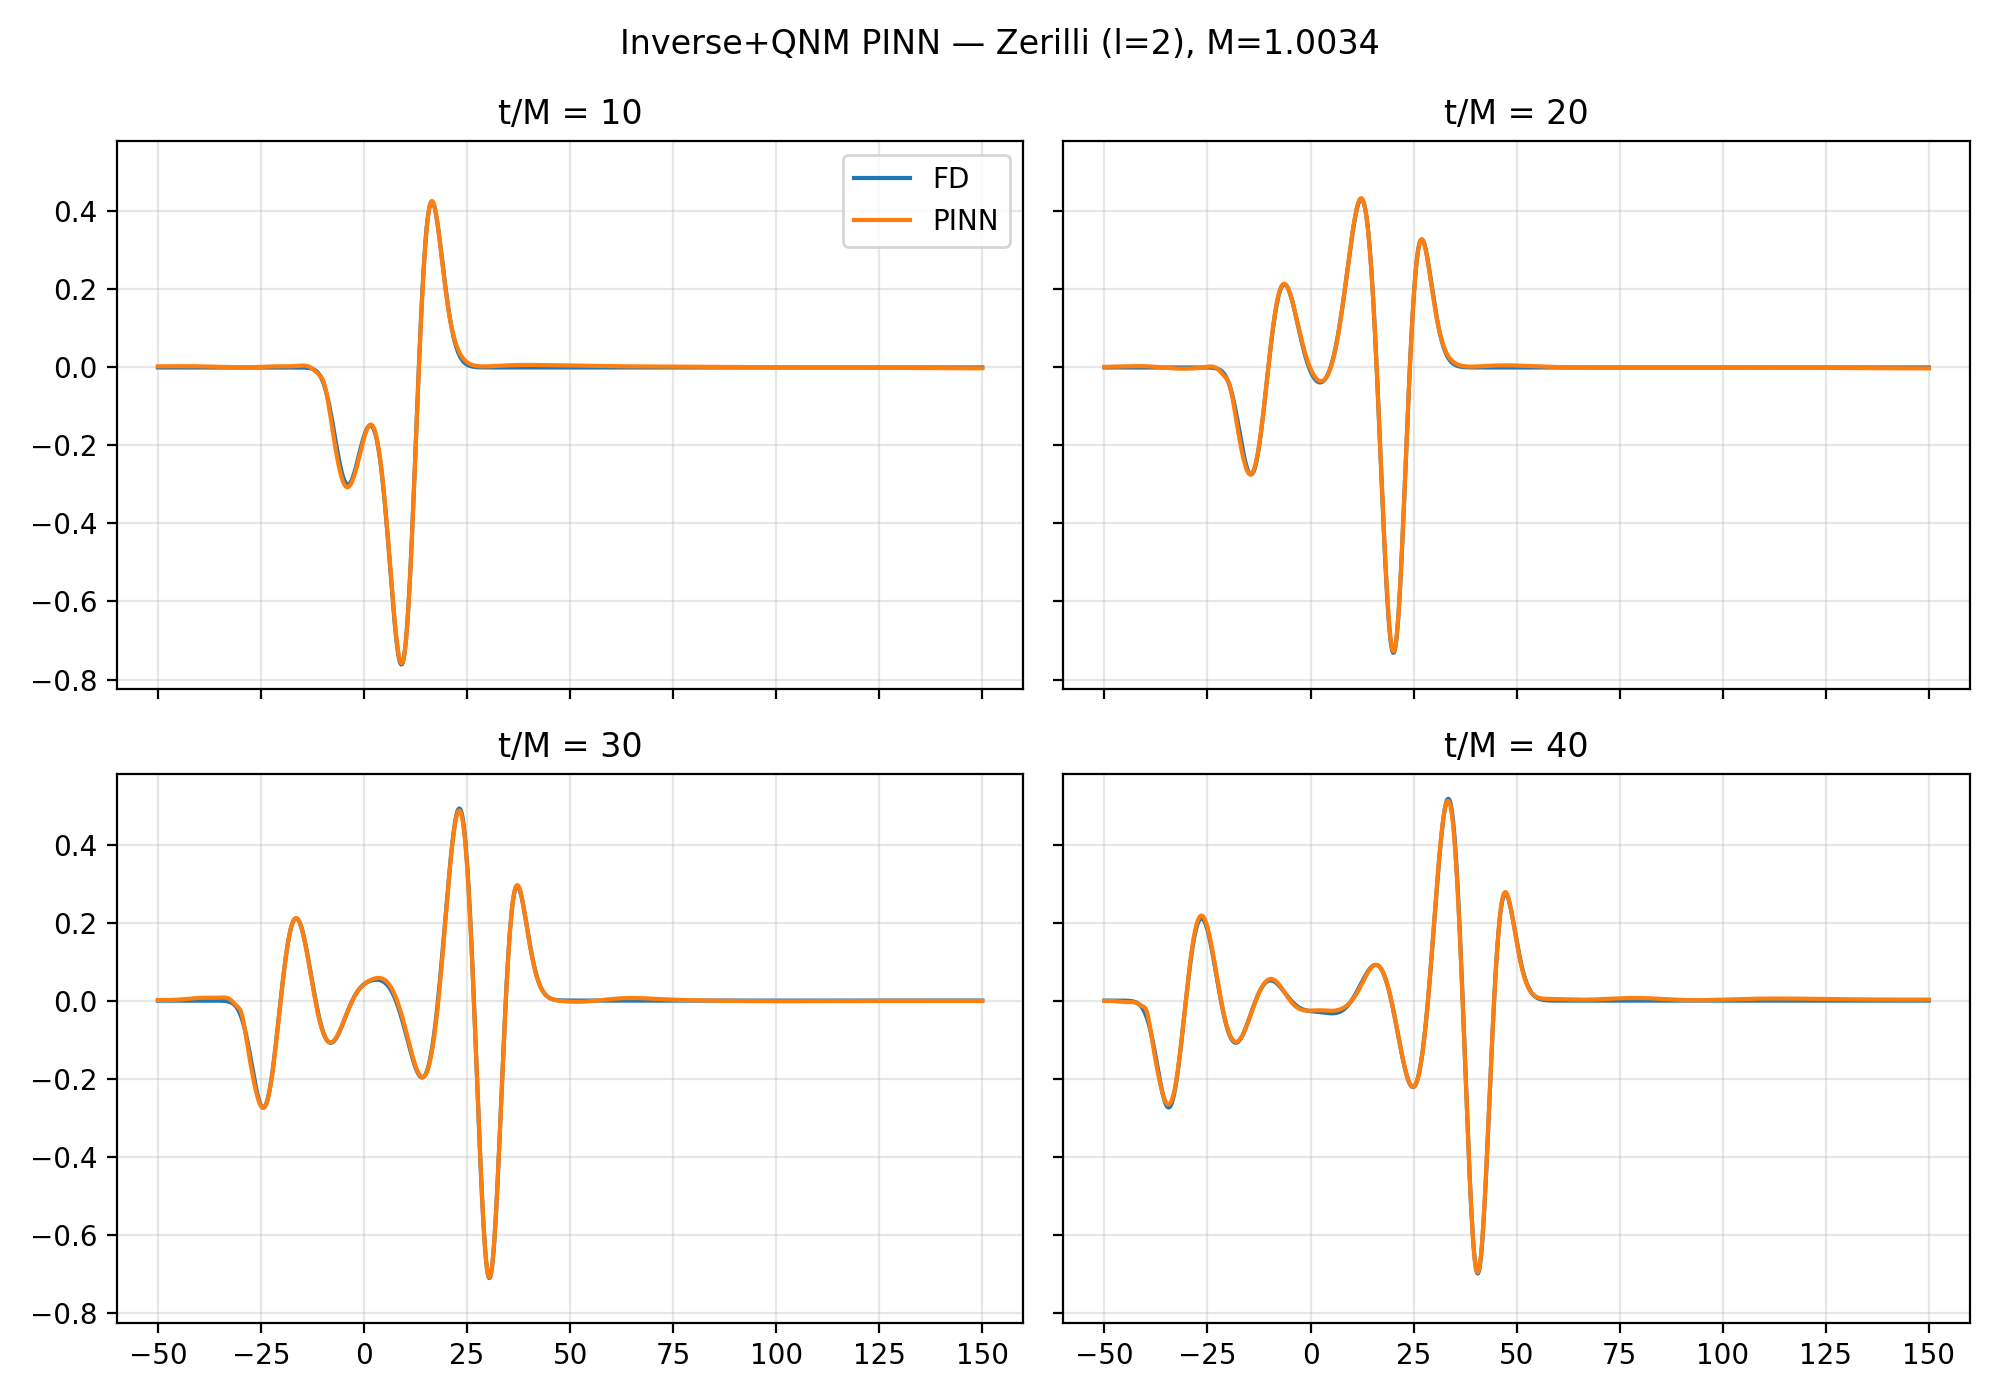
\includegraphics[width=\textwidth,height=0.72\textheight,keepaspectratio]{../outputs/pinn/zerilli_l2_inverse_qnm_combo/snapshots.png}
      \\[2pt]{\scriptsize Inverse PINN $\Phi_\theta$ (solid) vs.\ $\Phi_{\fd{}}$ (dashed)
      at $t/M\!\in\!\{10,20,30,40\}$, with $M$ treated as unknown.}
    \end{column}
    \begin{column}{0.48\textwidth}
      \centering
      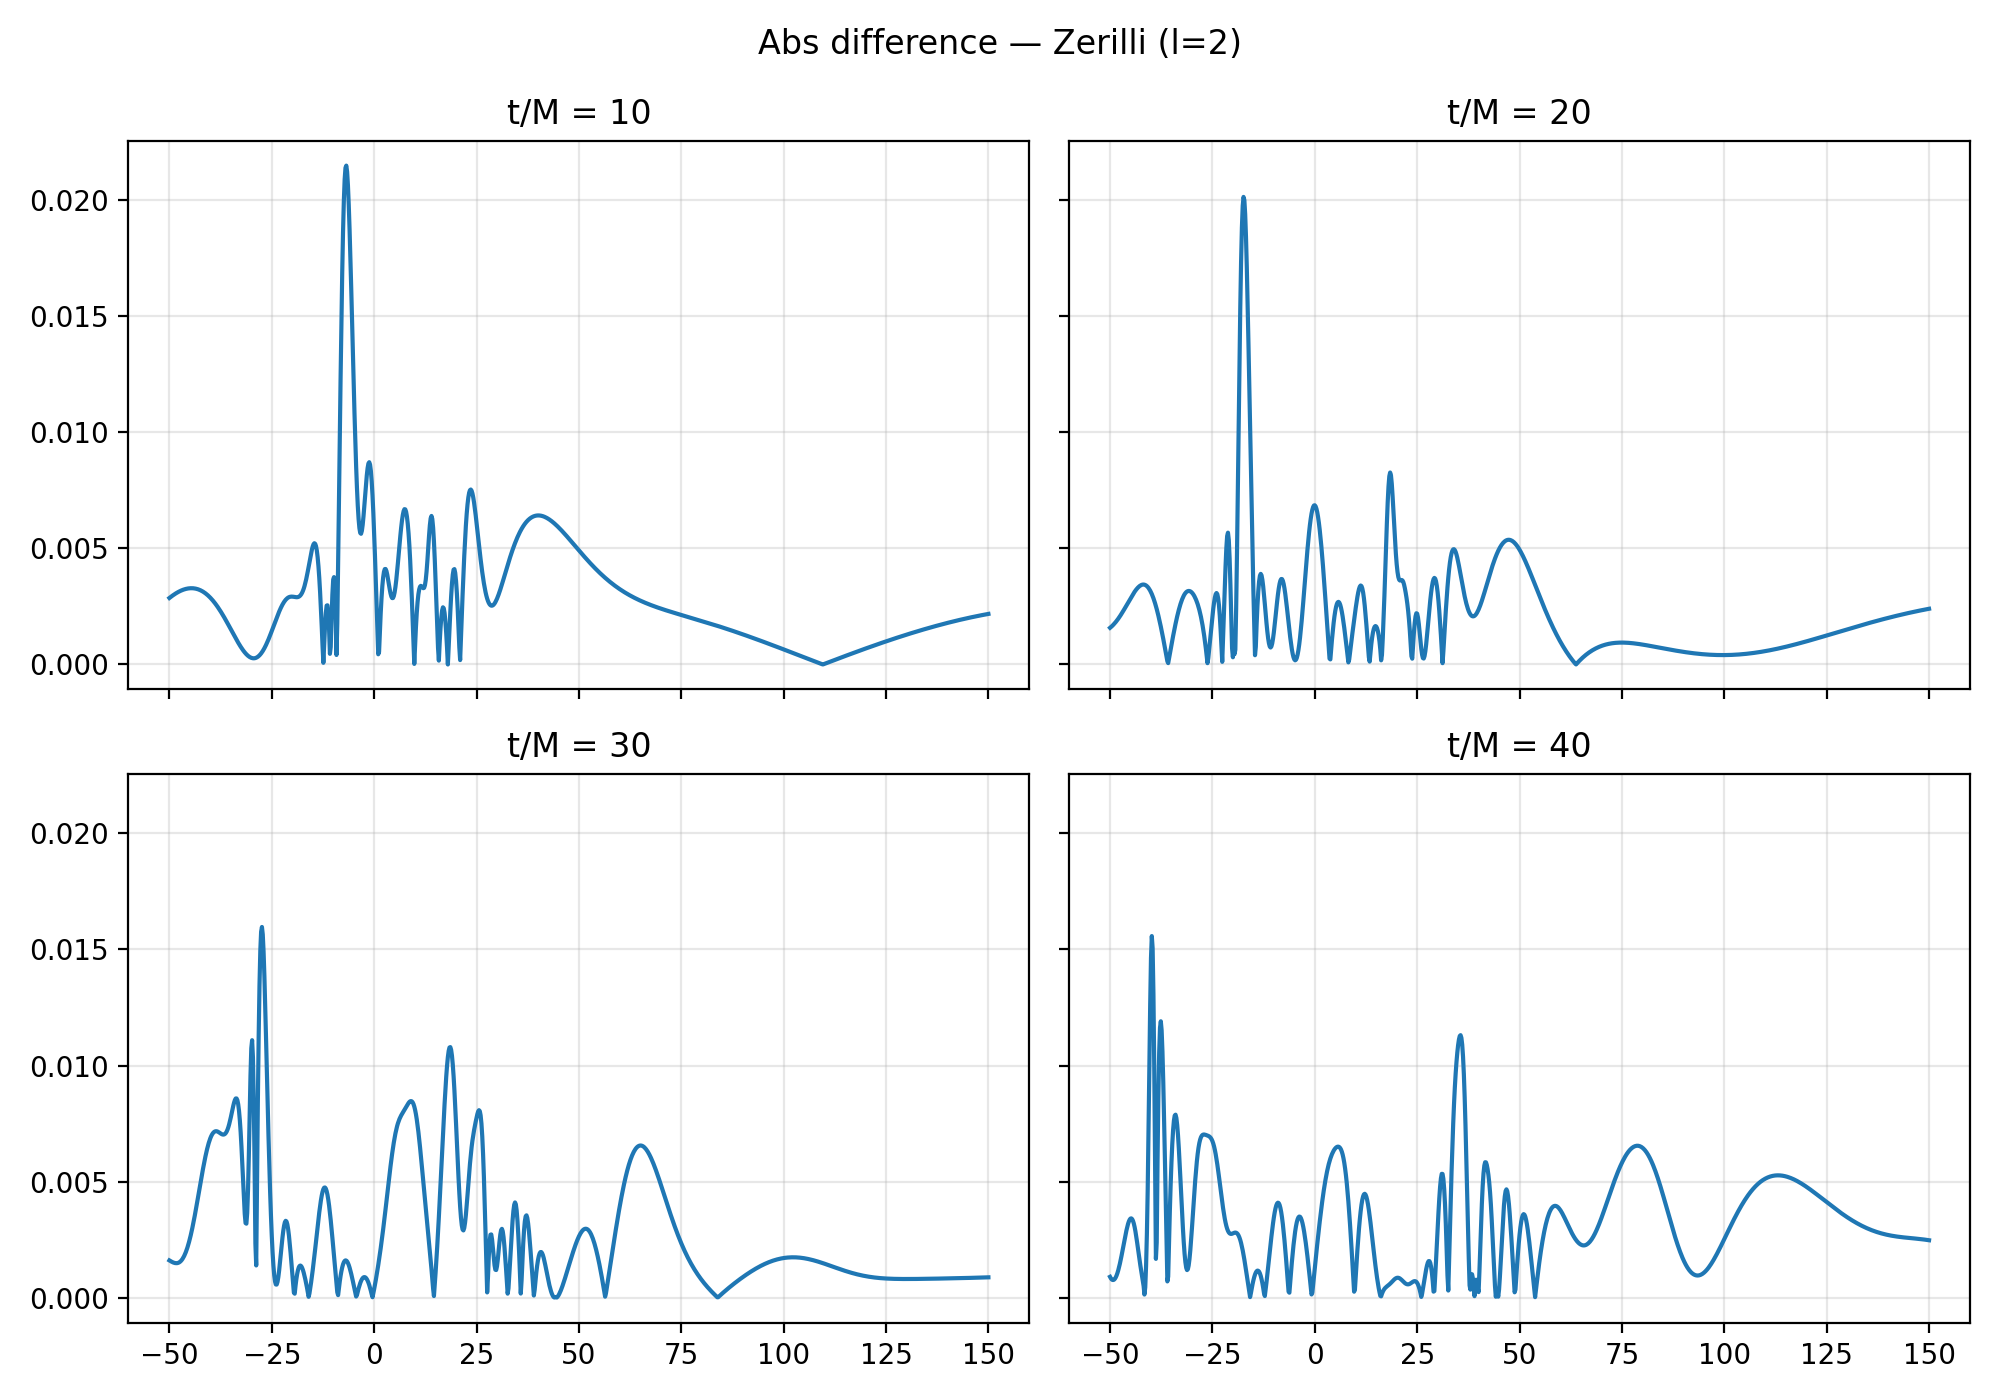
\includegraphics[width=\textwidth,height=0.72\textheight,keepaspectratio]{../outputs/pinn/zerilli_l2_inverse_qnm_combo/abs_diff_snapshots.png}
      \\[2pt]{\scriptsize Pointwise $|\Phi_\theta-\Phi_{\fd{}}|$ at the same times;
      waveform recovery comparable to the forward run while $M$ is
      simultaneously inferred to $0.34\%$.}
    \end{column}
  \end{columns}
\end{frame}

\begin{frame}{Inverse PINN --- parameter convergence}
  \begin{columns}[T]
    \begin{column}{0.62\textwidth}
      \centering
      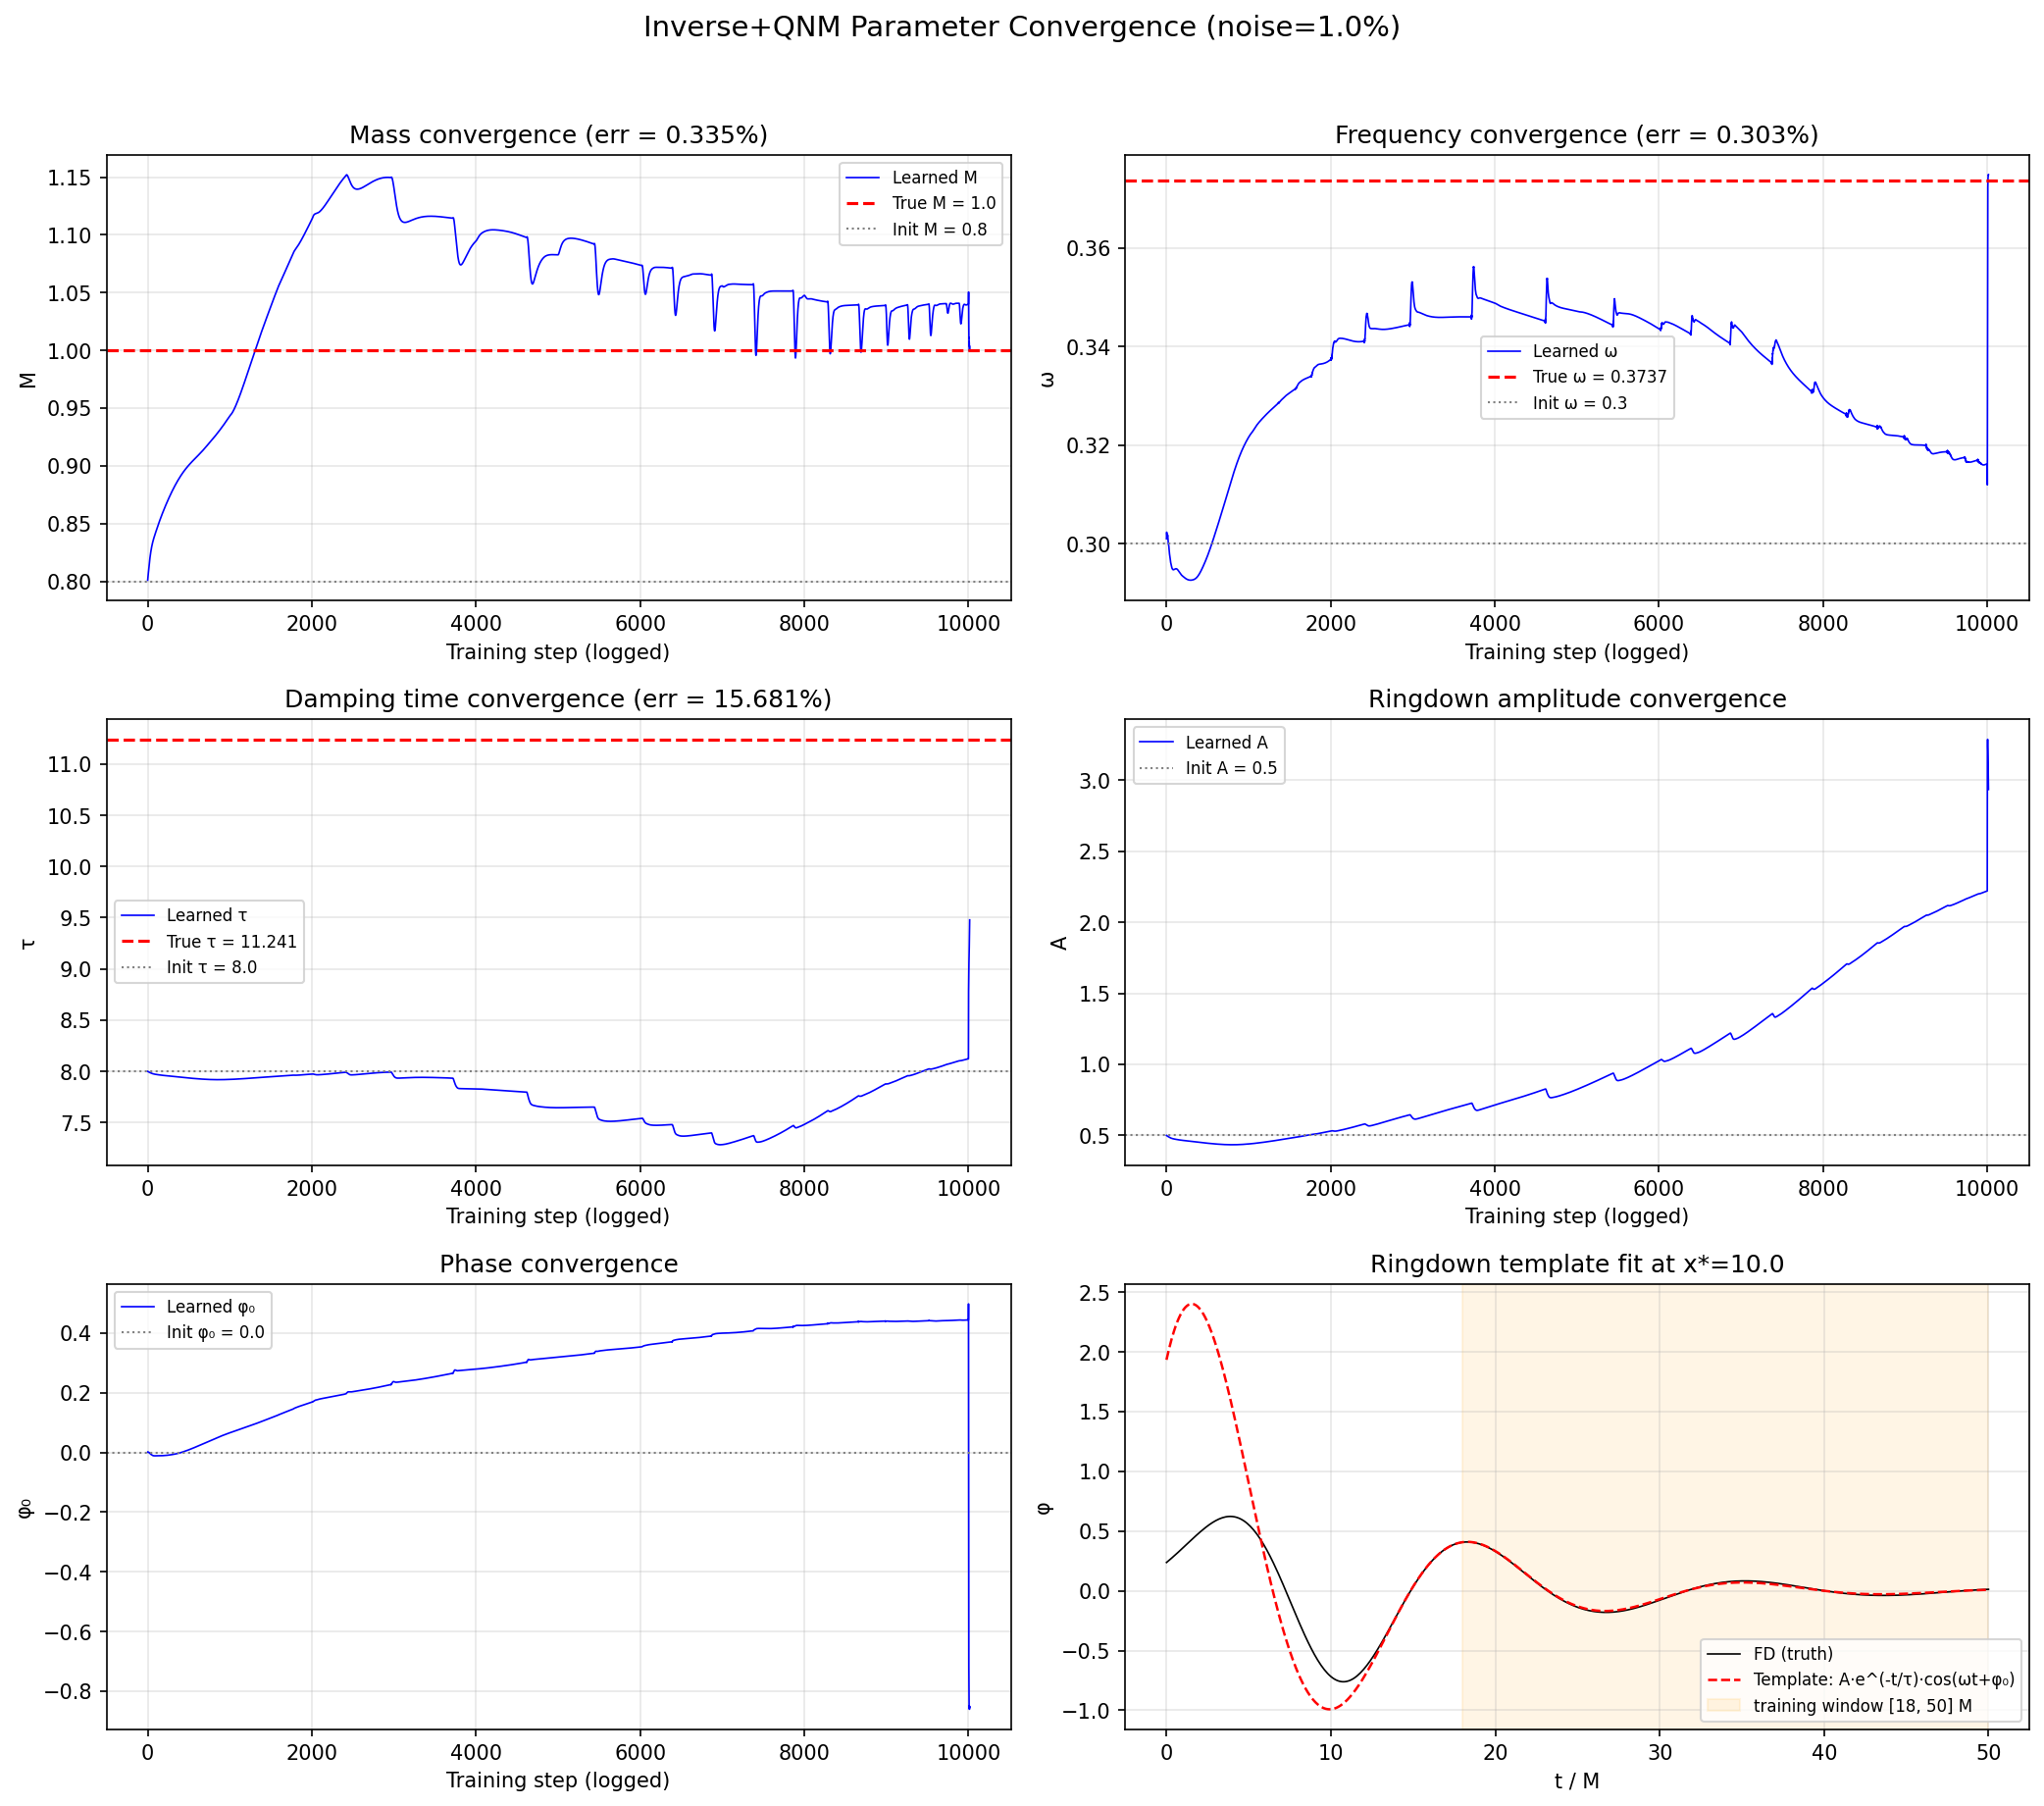
\includegraphics[width=\textwidth,height=0.78\textheight,keepaspectratio]{../outputs/pinn/zerilli_l2_inverse_qnm_combo/param_convergence.png}
    \end{column}
    \begin{column}{0.36\textwidth}
      \footnotesize
      Trajectories of the trainable scalars during Adam$\,\to\,$L-BFGS:
      \begin{itemize}
        \item $M\!:\;1.20\!\to\!1.0034$
        \item $\omega\!:\;0.30\!\to\!0.3748$
        \item $\tau\!:\;8.00\!\to\!11.06$
        \item $A_{\mathrm{ring}},\phi$ co-fit on the
              $[t_{\mathrm{ring}}^{\min},t_{\max}]$ window.
      \end{itemize}
      All five physical scalars settle inside the L-BFGS phase, with no
      observed parameter drift after convergence.
    \end{column}
  \end{columns}
\end{frame}

\begin{frame}{Inverse PINN --- best result: recovered parameters}
  \centering
  \renewcommand{\arraystretch}{1.25}
  \begin{tabular}{@{}lcccc@{}}
    \toprule
    \textbf{Parameter} & \textbf{Init} & \textbf{Learned} & \textbf{True} & \textbf{Error} \\
    \midrule
    $M$              & 1.20 & 1.0034 & 1.0    & \textcolor{darkgreen}{\textbf{0.34\%}} \\
    $\omega$ (M4 plateau)            & 0.30 & 0.3748 & 0.3737 & \textcolor{darkgreen}{\textbf{0.31\%}} \\
    $\tau$  (M2, window $[10,50]M$)  & 8.00 & 11.06  & 11.241 & \textcolor{darkgreen}{\textbf{1.59\%}} \\
    \bottomrule
  \end{tabular}
  \vspace{6mm}

  \fbox{\parbox{0.85\textwidth}{\centering
    \textbf{Variant D combo} hyperparameters:
    $t_{\text{ring}}^{\min}\!=\!18M$,\;
    $\lambda_{\text{ring}}\!=\!100$,\;
    $N_{\text{ring}}\!=\!1000$.\\
    \textbf{All three physical parameters recovered to $\le\!1.6\%$ in a single training run.}}}
\end{frame}


% ══════════════════════════════════════════════════════════════════
\section{4. Curriculum PINN}
% ══════════════════════════════════════════════════════════════════

\begin{frame}{Curriculum PINN --- problem statement}
  \textbf{Diagnosis.} The forward PINN's pointwise error grows
  monotonically with $t$: the late-time band $t\!\in\![37.5,50]M$
  contributes $\sim\!41\%$ of the full-domain RMSD, despite spanning
  only a quarter of the temporal domain.
  \medskip

  \textbf{Idea.} Replace the single-window forward PINN with a
  \emph{curriculum} [Bengio et al.\ 2009; Krishnapriyan et al.\ 2021]:
  split $t\!\in\![0,50]M$ into $K$ contiguous windows
  $W_{k}=[t_{k-1},t_{k}]$ and train an \emph{independent} PINN
  $\Phi_{\theta_{k}}$ on each, with the network of window $k$ supplying
  the initial conditions of window $k\!+\!1$:
  \[
    \Phi^{\mathrm{IC}}_{k}(x) = \Phi_{\theta_{k-1}}(x,t_{k-1}),\qquad
    \partial_{t}\Phi^{\mathrm{IC}}_{k}(x)
       = \partial_{t}\Phi_{\theta_{k-1}}(x,t_{k-1}).
  \]
  \medskip

  \textbf{Trade-off.}
  \begin{itemize}\small
    \item \textcolor{darkgreen}{\textbf{Pro:}} smaller temporal sub-domain $\Rightarrow$
          easier optimisation landscape per window.
    \item \textcolor{darkred}{\textbf{Con:}} every window after the first inherits
          the residual error of its predecessor through its IC.
  \end{itemize}
\end{frame}

\begin{frame}{Curriculum PINN --- three partitions}
  \centering
  \resizebox{0.95\textwidth}{!}{%
  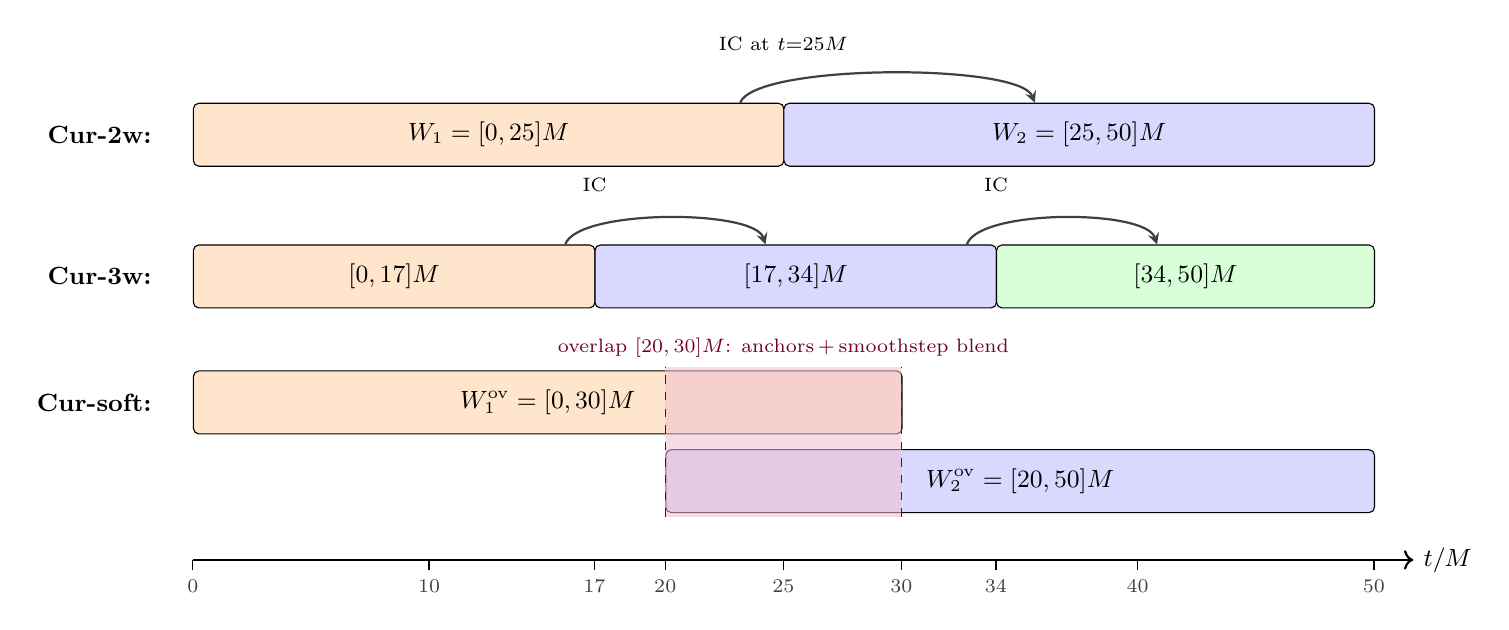
\begin{tikzpicture}[
    every node/.style={font=\small},
    win/.style={draw, rounded corners=2pt, minimum height=8mm,
                inner sep=2pt, font=\small},
    arr/.style={->, >=stealth, thick, gray!50!black},
    tick/.style={font=\scriptsize, gray!50!black},
  ]
    \def\sc{0.30}
    \def\xo{-0.5*50*\sc}

    % Cur-2w
    \node[font=\small\bfseries, anchor=east] at ({\xo - 0.4}, 2.4) {Cur-2w:};
    \node[win, fill=orange!20, minimum width={25*\sc cm}, anchor=west] (a1)
         at ({0*\sc + \xo}, 2.4) {$W_{1}=[0,25]M$};
    \node[win, fill=blue!15, minimum width={25*\sc cm}, anchor=west] (a2)
         at ({25*\sc + \xo}, 2.4) {$W_{2}=[25,50]M$};
    \draw[arr] ($(a1.north)!0.85!(a1.north east)$)
            .. controls +(0.2,0.5) and +(-0.2,0.5) ..
               ($(a2.north)!0.15!(a2.north west)$);
    \node[font=\scriptsize, anchor=south]
         at ({25*\sc + \xo}, 3.35) {IC at $t{=}25M$};

    % Cur-3w
    \node[font=\small\bfseries, anchor=east] at ({\xo - 0.4}, 0.6) {Cur-3w:};
    \node[win, fill=orange!20, minimum width={17*\sc cm}, anchor=west] (b1)
         at ({0*\sc + \xo}, 0.6) {$[0,17]M$};
    \node[win, fill=blue!15,   minimum width={17*\sc cm}, anchor=west] (b2)
         at ({17*\sc + \xo}, 0.6) {$[17,34]M$};
    \node[win, fill=green!15,  minimum width={16*\sc cm}, anchor=west] (b3)
         at ({34*\sc + \xo}, 0.6) {$[34,50]M$};
    \draw[arr] ($(b1.north)!0.85!(b1.north east)$)
            .. controls +(0.15,0.45) and +(-0.15,0.45) ..
               ($(b2.north)!0.15!(b2.north west)$);
    \draw[arr] ($(b2.north)!0.85!(b2.north east)$)
            .. controls +(0.15,0.45) and +(-0.15,0.45) ..
               ($(b3.north)!0.15!(b3.north west)$);
    \node[font=\scriptsize, anchor=south] at ({17*\sc + \xo}, 1.55) {IC};
    \node[font=\scriptsize, anchor=south] at ({34*\sc + \xo}, 1.55) {IC};

    % Cur-soft: two staggered rows + overlap band
    \node[font=\small\bfseries, anchor=east] at ({\xo - 0.4}, -1.0) {Cur-soft:};
    \node[win, fill=orange!20, minimum width={30*\sc cm}, anchor=west] (c1)
         at ({0*\sc + \xo}, -1.0) {$W_{1}^{\mathrm{ov}}=[0,30]M$};
    \node[win, fill=blue!15, minimum width={30*\sc cm}, anchor=west] (c2)
         at ({20*\sc + \xo}, -2.0) {$W_{2}^{\mathrm{ov}}=[20,50]M$};
    \fill[purple!25, opacity=0.55]
         ({20*\sc + \xo}, -2.45) rectangle ({30*\sc + \xo}, -0.55);
    \draw[purple!60!black, dashed] ({20*\sc + \xo}, -2.45) -- ({20*\sc + \xo}, -0.55);
    \draw[purple!60!black, dashed] ({30*\sc + \xo}, -2.45) -- ({30*\sc + \xo}, -0.55);
    \node[font=\scriptsize, anchor=south, purple!60!black]
         at ({25*\sc + \xo}, -0.55)
         {overlap $[20,30]M$: anchors\,+\,smoothstep blend};

    % Time axis
    \draw[->, thick] ({0*\sc + \xo}, -3.0)
                  -- ({50*\sc + \xo + 0.5}, -3.0) node[right]{$t/M$};
    \foreach \t in {0,10,17,20,25,30,34,40,50}{
      \draw ({\t*\sc + \xo}, -3.0) -- ({\t*\sc + \xo}, -3.13);
      \node[tick, below] at ({\t*\sc + \xo}, -3.13) {\t};
    }
  \end{tikzpicture}}
  \\[6pt]
  \begin{minipage}{0.92\textwidth}
    \centering\scriptsize
    \textbf{Cur-2w} and \textbf{Cur-3w}: hard partition --- IC of each window
    extracted from the previous network at the splice time.
    \textbf{Cur-soft}: overlapping windows with continuity anchors and a
    smoothstep blend on the overlap band (next slide).
  \end{minipage}
\end{frame}

\begin{frame}{Curriculum PINN --- loss per window}
  \footnotesize
  Each window $W_{k}$ minimises the \textbf{same seven-term forward loss}
  as the forward PINN, evaluated on $W_{k}$ only:
  \[
    \mathcal{L}_{\mathrm{cur},k}
    \;=\;
    \underbrace{\textcolor{darkred}{\lambda_{r}\mathcal{L}_{r}^{(k)}
      + \lambda_{r_{x}}\mathcal{L}_{r_{x}}^{(k)}
      + \lambda_{r_{t}}\mathcal{L}_{r_{t}}^{(k)}}}_{\text{PDE residual + gPINN on }W_{k}}
    \;+\;
    \underbrace{\textcolor{darkgreen}{\lambda_{\mathrm{ic}}\mathcal{L}_{\mathrm{ic}}^{(k)}
      + \lambda_{\mathrm{iv}}\mathcal{L}_{\mathrm{iv}}^{(k)}}}_{\text{IC at }t=t_{k-1}}
    \;+\;
    \underbrace{\textcolor{blue}{\lambda_{\mathrm{bl}}\mathcal{L}_{\mathrm{bl}}^{(k)}
      + \lambda_{\mathrm{br}}\mathcal{L}_{\mathrm{br}}^{(k)}}}_{\text{boundary conditions}}
  \]
  \medskip

  \textcolor{darkgreen}{\textbf{Initial condition losses}} differ by window:
  \begin{itemize}
    \item \textbf{Window 1} ($k\!=\!1$): same analytic Gaussian-pulse IC as
          the forward PINN,
          $\mathcal{L}_{\mathrm{ic}}^{(1)} \!=\! \frac{1}{N_{\mathrm{ic}}}
          \sum_j[\Phi_{\theta_{1}}(x_j,0) - \Phi_{0}(x_j)]^{2}$,
          $\;\mathcal{L}_{\mathrm{iv}}^{(1)} \!=\! \frac{1}{N_{\mathrm{ic}}}
          \sum_j[\partial_t\Phi_{\theta_{1}}(x_j,0)]^{2}$.

    \item \textbf{Window $k\!\ge\!2$}: IC extracted from the \emph{trained}
          previous network $\Phi_{\theta_{k-1}}$ at the splice time $t_{k-1}$:
          \[
            \textcolor{darkgreen}{\mathcal{L}_{\mathrm{ic}}^{(k)}}
            = \frac{1}{N_{\mathrm{ic}}}\sum_{j}
              \bigl[\Phi_{\theta_{k}}(x_{j},t_{k-1})
                    - \Phi_{\theta_{k-1}}(x_{j},t_{k-1})\bigr]^{2}
          \]
          \[
            \textcolor{darkgreen}{\mathcal{L}_{\mathrm{iv}}^{(k)}}
            = \frac{1}{N_{\mathrm{ic}}}\sum_{j}
              \bigl[\partial_{t}\Phi_{\theta_{k}}(x_{j},t_{k-1})
                    - \partial_{t}\Phi_{\theta_{k-1}}(x_{j},t_{k-1})\bigr]^{2}
          \]
  \end{itemize}
  All weights $\boldsymbol{\lambda}$ and the (Adam $10{,}000$ + L-BFGS $30{,}000$)
  schedule are identical to the forward PINN, applied independently per window.
\end{frame}

\begin{frame}{Curriculum PINN --- soft-overlap variant}
  \footnotesize
  Two windows share an overlap band of width $\Delta_{\mathrm{ov}}$
  centred on $t_{\mathrm{split}}$:
  \[
    W_{1}^{\mathrm{ov}}=[t_{\min},t_{\mathrm{split}}+\Delta_{\mathrm{ov}}/2],\quad
    W_{2}^{\mathrm{ov}}=[t_{\mathrm{split}}-\Delta_{\mathrm{ov}}/2,t_{\max}].
  \]
  \medskip

  \textcolor{purple}{\textbf{Continuity-anchor loss}} on a fixed
  $n_{x}\!\times\!n_{t}$ grid spanning the overlap rectangle:
  \[
    \textcolor{purple}{\mathcal{L}_{\mathrm{cont}}}
    = \frac{\lambda_{\mathrm{cont}}}{n_{x} n_{t}}
      \sum_{i,j}\bigl(\Phi_{\theta_{2}}(x_{i},t_{j})-\Phi_{\theta_{1}}(x_{i},t_{j})\bigr)^{2},
  \]
  added to $\Phi_{\theta_{2}}$'s loss; pulls window 2 towards the
  already-trained window 1 across the entire overlap rather than
  at the splice time alone.
  \medskip

  \textcolor{darkgreen}{\textbf{Smoothstep blend}} on the overlap band:
  \[
    \Phi_{\mathrm{cur}}^{\mathrm{ov}}(x,t)
    = \bigl(1-s(\xi)\bigr)\,\Phi_{\theta_{1}} + s(\xi)\,\Phi_{\theta_{2}},
    \quad s(\xi)=\xi^{2}(3-2\xi),\quad
    \xi=\frac{t-t_{\mathrm{ov}}^{-}}{\Delta_{\mathrm{ov}}}.
  \]
  $s$ is $C^{1}$ with $s(0)\!=\!0$, $s(1)\!=\!1$, $s'(0)\!=\!s'(1)\!=\!0$
  $\Rightarrow$ stitched field is continuously differentiable across the
  overlap edges.
  \medskip

  \textbf{Settings.} $\Delta_{\mathrm{ov}}\!=\!10M$,
  $n_{x}\!\times\!n_{t}\!=\!201\!\times\!11$,
  $\lambda_{\mathrm{cont}}\!=\!10$.
\end{frame}

\begin{frame}{Curriculum PINN --- variants and results}
  \centering\scriptsize
  \renewcommand{\arraystretch}{1.05}
  \begin{tabular}{@{}lcccc@{}}
    \toprule
    \textbf{Variant} & \textbf{Full-domain RMSD} & $W_{1}$ \textbf{RMSD}
                     & $W_{2}$ \textbf{RMSD} & $W_{3}$/overlap \textbf{RMSD} \\
                     & ($\times 10^{-3}$) & ($\times 10^{-3}$) & ($\times 10^{-3}$) & ($\times 10^{-3}$) \\
    \midrule
    Baseline (single window) & \textbf{0.817} & --- & --- & --- \\
    \midrule
    Cur-2w   & 0.845 & \textbf{0.516} & 1.077 & --- \\
    Cur-3w   & 0.976 & 0.554          & 0.920 & 1.322 \\
    Cur-soft & 3.155 & 1.739          & 3.932 & 2.394 (overlap) \\
    \bottomrule
  \end{tabular}
  \vspace{2mm}

  \begin{itemize}\scriptsize
    \item \textbf{Cur-2w ties baseline} on full domain ($+3\%$); $W_{1}$ alone
          reaches $5.16\!\times\!10^{-4}$ ($-37\%$ vs.\ baseline on the same
          sub-domain) --- the predicted local benefit \emph{is} delivered.
    \item \textbf{Cur-3w}: per-window RMSD grows monotonically
          ($5.5\!\to\!9.2\!\to\!13.2$); each splice adds IC error.
          Full-domain $+19\%$.
    \item \textbf{Cur-soft fails:} $\sim\!4\times$ baseline RMSD; M4 plateau
          scan finds no contiguous block satisfying the relative-scatter criterion.
  \end{itemize}

  \fbox{\parbox{0.92\textwidth}{\centering\scriptsize
    \textbf{Take-away.} Curriculum buys local accuracy on $W_{1}$ but pays
    it back through IC-transfer error on later windows; no net gain over
    the single-window forward PINN.}}
\end{frame}


% ══════════════════════════════════════════════════════════════════
\section{5. Extraction methods M3, M4, M5}
% ══════════════════════════════════════════════════════════════════

\begin{frame}{Why we need new extraction methods}
  Patel et al.\ 2024 (and our earlier work) used:
  \medskip
  \begin{itemize}
    \item \textbf{M1 --- FFT + log-linear envelope:}
          $\omega$ from FFT peak, $\tau$ from $\log|\text{peaks}|$ slope.
    \item \textbf{M2 --- single-mode NLS curve fit:}
          fit $A e^{-t/\tau}\cos(\omega t+\phi)$ over a chosen window.
  \end{itemize}
  \medskip
  \textbf{Two unsolved problems with M1/M2:}
  \begin{enumerate}\small
    \item \textbf{Overtone contamination.} The first overtone
          $\tau_{1}\!=\!3.67\,M$ is comparable to the burst at early times.
          A single-mode fit absorbs it as bias.
    \item \textbf{Window dependence.} M1 and M2 quote a single number
          from a single window, with no estimate of how that number
          changes if the window edges move. \textbf{This is not a falsifiable
          measurement.}
  \end{enumerate}
  \medskip
  \textbf{M3, M4, M5} are our advances that address both.
\end{frame}

\begin{frame}{M3 --- ESPRIT subspace decomposition}
  \textbf{Idea:} treat the ringdown as a sum of $K$ complex exponentials
  and solve for them \emph{simultaneously} using subspace methods
  (Estimation of Signal Parameters via Rotational Invariance Techniques).
  \medskip
  \[
    \Phi(x_{q},t)
    \;\approx\; \sum_{k=1}^{K} A_{k}\,e^{(i\omega_{k} - 1/\tau_{k})\,t}
  \]
  \medskip
  \textbf{Procedure:}
  \begin{enumerate}\small
    \item Optionally Hilbert-transform the real signal to its analytic
          (complex) form so each physical mode appears once.
    \item Build the Hankel data matrix; SVD to get the signal subspace.
    \item Solve the rotational-invariance eigenvalue problem
          $\;\mathbf{U}_{1}^{\dagger}\mathbf{U}_{2} = \boldsymbol{\Psi}$.
    \item Eigenvalues of $\boldsymbol{\Psi}$ $\to$ $(\omega_{k}, \tau_{k})$;
          report the largest-amplitude mode.
  \end{enumerate}
  \medskip
  \textbf{Strength:} no initial guess; resolves multiple modes naturally.\\
  \textbf{Weakness:} sensitive to Hankel-matrix conditioning at low SNR;
  on inverse-PINN waveforms can become ill-conditioned.
\end{frame}

\begin{frame}{M4 --- two-mode NLS with start-time plateau scan}
  \textbf{Step 1.} Fit a \emph{two-mode} template (fundamental + first overtone):
  \[
    \Phi_{\text{model}}(t)
    \;=\;
    A_{0}\,e^{-t/\tau_{0}}\cos(\omega_{0}t+\phi_{0})
    \;+\;
    A_{1}\,e^{-t/\tau_{1}}\cos(\omega_{1}t+\phi_{1})
  \]
  using \texttt{scipy.optimize.curve\_fit} with bound constraints,
  on window $[t_{0},\,t_{\max}]$.
  Identify the longer-$\tau$ mode as the fundamental.
  \medskip

  \textbf{Step 2.} Repeat over a grid of start times $t_{0}\in[10,25]M$.
  Identify the contiguous \textbf{plateau} of low-scatter
  consecutive fits.
  \medskip

  \textbf{Step 3.} Report:
  \[
    \omega_{\!_{M4}} \;=\; \langle\omega\rangle_{\text{plateau}},
    \qquad
    \sigma_{\omega} \;=\; \mathrm{std}(\omega)_{\text{plateau}}
  \]
  --- the plateau spread is a \textbf{principled systematic error bar}.
  \medskip

  \textbf{Why it works:} an honest QNM extraction must be invariant to small
  shifts of the fit window; the plateau is the empirical signature of
  that invariance.
\end{frame}

\begin{frame}{M4 --- example stability scan}
  \begin{columns}[T]
    \begin{column}{0.52\textwidth}
      \centering
      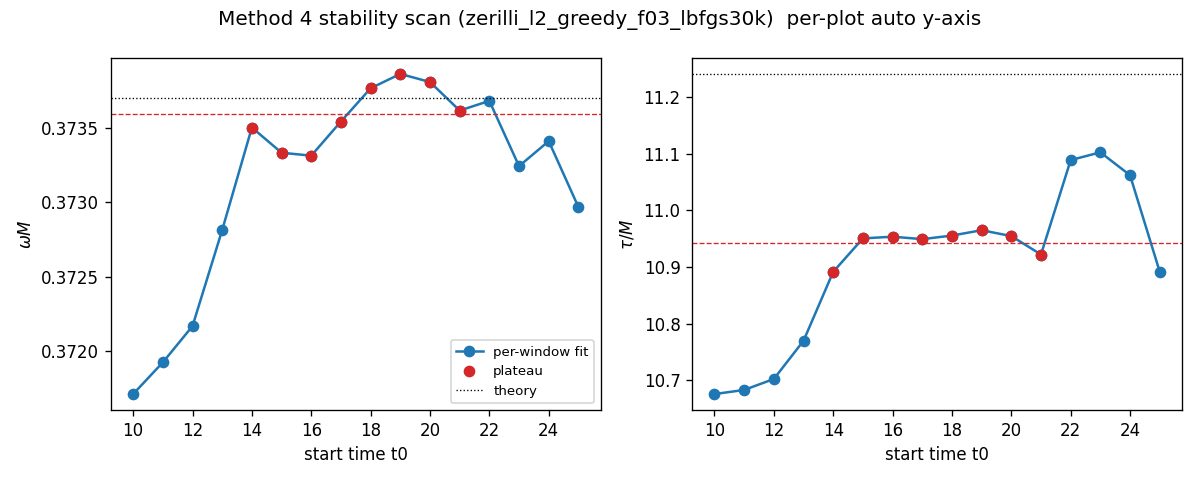
\includegraphics[width=\textwidth,height=0.78\textheight,keepaspectratio]{../outputs/qnm/zerilli_l2_greedy_f03_lbfgs30k/pinn_method4_stability.png}
      \\{\footnotesize Forward PINN: M4 stability scan over $t_{0}\in[10,25]M$}
    \end{column}
    \begin{column}{0.46\textwidth}
      \begin{itemize}\small
        \item $\omega$ (top): essentially flat across most of $t_{0}\in[14,21]M$
              $\;\Rightarrow\;$ plateau identified.
        \item $\tau$ (bottom): converges to a stable value once $t_{0}$ is past the
              prompt burst.
        \item Plateau quote:
              $\omega_{\!_{M4}} = 0.37359 \pm 1.96\times10^{-4}$
              $\;\Rightarrow\;$ $0.029\%$ error vs.\ Leaver.
        \item Vertical span of the green band $= 2\sigma_{\omega}$ ---
              an honest, falsifiable systematic.
      \end{itemize}
    \end{column}
  \end{columns}
\end{frame}

\begin{frame}{M5 --- two-mode NLS with 2-D plateau scan}
  M4 sweeps only one window edge ($t_{0}$). \textbf{M5} sweeps both:
  \[
    [t_{0},\, t_{\text{end}}] \;\in\; [10,25]M \times [t_{\min},\,50]M
    \quad\text{on a $10\!\times\!6$ grid.}
  \]
  Identify the contiguous \textbf{rectangular plateau} of $5\!\times\!3$
  with smallest combined relative scatter; report plateau-mean and
  plateau-stddev.
  \medskip

  \textbf{Why this matters:}
  \begin{itemize}\small
    \item $t_{0}$ scans control \emph{overtone leakage} (early edge).
    \item $t_{\text{end}}$ scans control \emph{Price tail leakage} (late edge).
    \item Truncating either edge prematurely is a model-misspecification
          bias, not a noise issue --- it does \emph{not} go away with more data.
    \item M5 is, to our knowledge, the \textbf{first systematic 2-D
          plateau analysis} applied to PINN-derived QNM extraction.
  \end{itemize}
\end{frame}

\begin{frame}{M5 --- example 2-D heatmap}
  \begin{columns}[T]
    \begin{column}{0.46\textwidth}
      \centering
      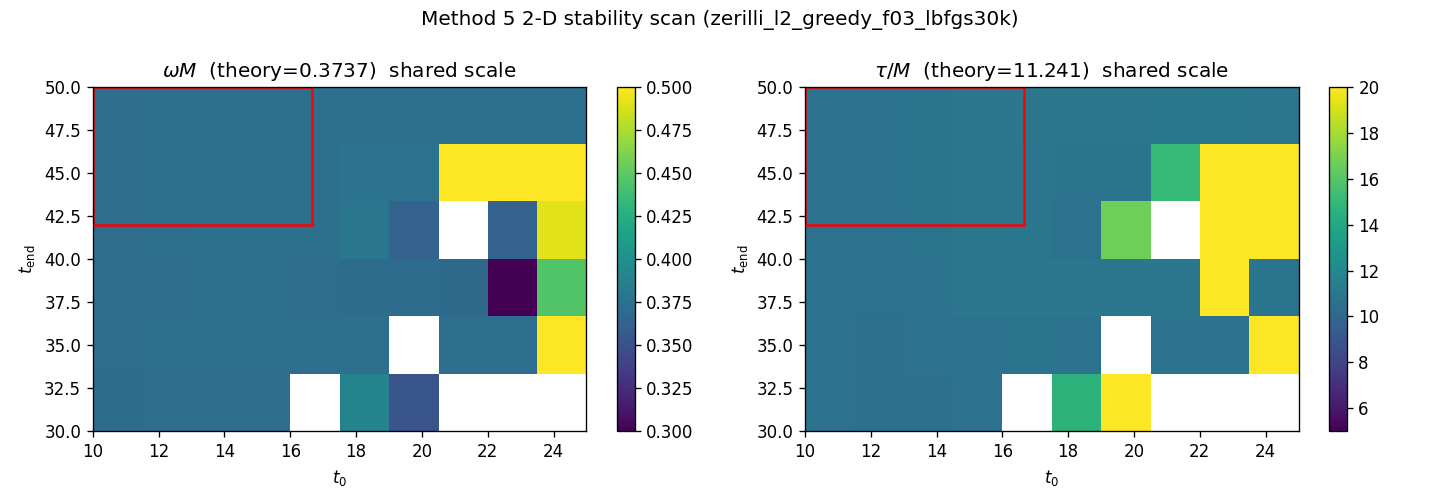
\includegraphics[width=\textwidth,height=0.80\textheight,keepaspectratio]{../outputs/qnm/zerilli_l2_greedy_f03_lbfgs30k/pinn_method5_2d_heatmap.png}
    \end{column}
    \begin{column}{0.52\textwidth}
      \footnotesize
      \textbf{Top:} $\omega$ scatter map. \textbf{Bottom:} $\tau$ scatter map.
      \begin{itemize}
        \item $x$-axis: $t_{0}$ (start of fit window).
        \item $y$-axis: $t_{\text{end}}$ (end of fit window).
        \item Colour: relative scatter inside the local rectangle (capped at $5\%$).
        \item \textcolor{red!75!black}{\textbf{Red box:}} plateau (minimum joint scatter).
        \item Grey: NaN cells where the two-mode fit failed.
      \end{itemize}
      \medskip
      \textbf{Plateau quote:}
      \[
        \omega_{\!_{M5}} = 0.3732 \;(\text{0.13\% bias}),\quad
        \tau_{\!_{M5}} = 10.82 \;(\text{3.91\% bias}).
      \]
      M5 reproduces M4 \emph{and} certifies the right-edge choice is
      harmless --- a property M4 alone cannot test.
    \end{column}
  \end{columns}
\end{frame}

\begin{frame}{Reporting convention --- best estimator per quantity}
  Different physical quantities are best estimated from different
  features of the waveform. We therefore quote a \textbf{hybrid headline}:
  \medskip
  \begin{center}\small
    \begin{tabular}{@{}lll@{}}
      \toprule
      \textbf{Quantity} & \textbf{Estimator} & \textbf{Reason} \\
      \midrule
      $\omega$ &
        \textbf{M4 plateau mean} &
        Phase information aggregated across cycles;\\
        & & lowest-variance estimator
        ($\sigma_{\omega}\!\sim\!10^{-5}$). \\
      \addlinespace
      $\tau$ &
        \textbf{M2 over wide window} $[10,50]M$ &
        Amplitude information over longest decay range; \\
        & & avoids early-edge overtone bias. \\
      \bottomrule
    \end{tabular}
  \end{center}
  \medskip
  \begin{itemize}\small
    \item This is consistent with established practice in numerical-relativity
          ringdown analysis (Berti et al.\ 2007).
    \item Patel et al.\ 2024 use a similar split (FFT for $\omega$,
          envelope for $\tau$) but report \emph{no fit-window sensitivity}.
    \item M3, M4, M5 are also reported as cross-checks; on healthy
          forward runs all three agree to within their plateau widths.
  \end{itemize}
\end{frame}

\begin{frame}{All extraction methods on the best forward PINN}
  \begin{center}\footnotesize
    \begin{tabular}{@{}lcccc@{}}
      \toprule
      \textbf{Method} & $\boldsymbol{\omega}$ & $\boldsymbol{\omega}$ \textbf{err} & $\boldsymbol{\tau}$ & $\boldsymbol{\tau}$ \textbf{err} \\
      \midrule
      Truth (Leaver)         & 0.3737  & ---     & 11.241 & ---     \\
      \midrule
      M1 (FFT + envelope)    & 0.3712  & 0.68\%  & 10.92  & 2.83\%  \\
      M2 (single-mode NLS)   & 0.3794  & 1.54\%  & 11.46  & 1.99\%  \\
      M3 (ESPRIT, $K\!=\!6$) & 0.4829  & 29.2\%  & 7.84   & 30.3\%  \\
      \rowcolor{green!10}
      M4 (two-mode plateau)  & 0.37359 & \textbf{0.029\%} & 10.94  & 2.65\%  \\
      M5 (2-D plateau)       & 0.37284 & 0.23\%  & 10.80  & 3.91\%  \\
      \bottomrule
    \end{tabular}
  \end{center}
  \medskip
  \begin{itemize}\small
    \item \textbf{M4 wins on $\omega$ by an order of magnitude} ---
          plateau scan + two-mode template removes both overtone bias
          and window-choice arbitrariness.
    \item \textbf{M3 fails} on this run: ESPRIT's Hankel matrix is
          ill-conditioned at low signal levels (max amp $\sim 10^{-24}$
          flagged automatically).
    \item M2 wide-window remains the best $\tau$ estimator.
    \item All methods are reported \emph{together} as the cross-check
          --- divergences flag waveform pathologies.
  \end{itemize}
\end{frame}


% ══════════════════════════════════════════════════════════════════
\section{6. Greedy adaptive resampling}
% ══════════════════════════════════════════════════════════════════

\begin{frame}{Why adaptive sampling matters}
  \begin{columns}[T]
    \begin{column}{0.50\textwidth}
      Uniform collocation wastes points where the residual is already small
      and starves the network where it is large.
      \medskip
      \begin{itemize}\small
        \item \textbf{Residual-Adaptive Distribution (RAD)}
              [Wu et al.\ 2023]: probabilistic resampling
              with $p_{i} \propto |r_{i}|^{k} + c$.
              Two hyperparameters ($k$, $c$).
        \item Stochastic $\;\Rightarrow\;$ extreme residuals
              are not always selected.
        \item Sampling noise can interfere with Adam dynamics.
      \end{itemize}
    \end{column}
    \begin{column}{0.48\textwidth}
      \centering
      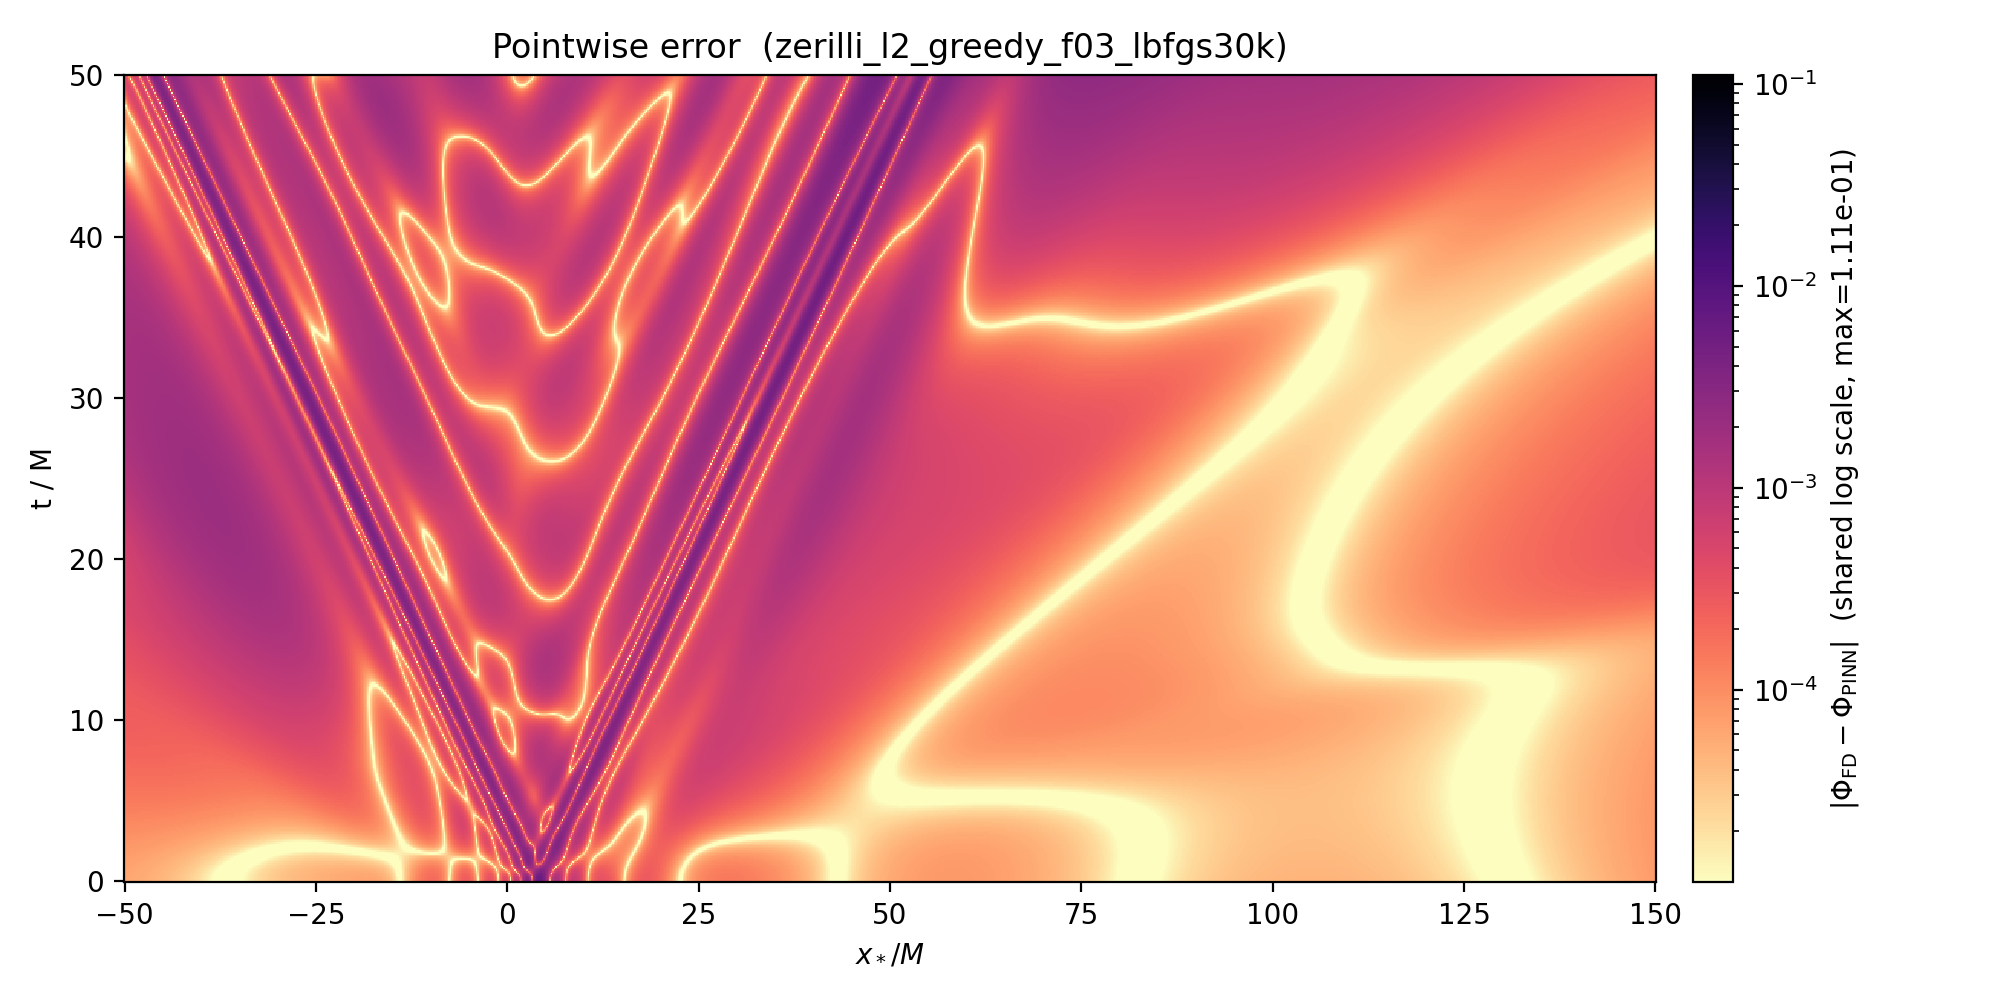
\includegraphics[width=\textwidth]{../outputs/pinn/zerilli_l2_greedy_f03_lbfgs30k/error_heatmap.png}
      \\{\footnotesize Final error map: PINN residual concentrates along
      the wavefronts that travel out from the burst.}
    \end{column}
  \end{columns}
\end{frame}

\begin{frame}{Greedy resampling --- algorithm}
  Replace probabilistic RAD with \textbf{deterministic top-$N$} selection:
  \medskip
  \begin{enumerate}\small
    \item Every $P$ Adam steps:
          generate $N_{\text{cand}}\!=\!100{,}000$ random candidates
          in the domain.
    \item Evaluate the PDE residual $|r_{i}|$ at each candidate
          (one extra forward pass --- batched, $\ll$ training cost).
    \item \textbf{Sort by $|r_{i}|$ descending}; keep the top
          $f \cdot N_{r}$ points.
    \item Fill the remaining $(1{-}f)\cdot N_{r}$ slots with
          \textbf{uniform random} points (preserves exploration).
    \item Replace all $N_{r}\!=\!32{,}000$ collocation points;
          continue Adam.
  \end{enumerate}
  \medskip
  \textbf{Key advantages over RAD:}
  \begin{itemize}\small
    \item \textbf{Deterministic} --- the worst residuals are always kept.
    \item \textbf{Single hyperparameter $f$.}
          $f\!=\!0$: uniform; $f\!=\!1$: fully greedy.
    \item No need to tune the $|r|^{k}+c$ shape.
  \end{itemize}
\end{frame}

\begin{frame}{Greedy resampling --- $f$ sweep results}
  \begin{columns}[T]
    \begin{column}{0.50\textwidth}
      \centering\footnotesize
      \begin{tabular}{@{}lcc@{}}
        \toprule
        \textbf{Configuration} & \textbf{RMSD} & \textbf{vs.\ baseline} \\
        \midrule
        Uniform (baseline)  & 0.00183 & --- \\
        RAD $k\!=\!2$       & 0.00095 & $-48\%$ \\
        \midrule
        Greedy $f\!=\!0.3$  & \textbf{0.00085} & \textbf{$-54\%$} \\
        Greedy $f\!=\!0.5$  & 0.00107 & $-42\%$ \\
        Greedy $f\!=\!0.8$  & 0.00165 & $-10\%$ \\
        \rowcolor{green!10}
        Greedy $f\!=\!0.3$\\
        \;+ L-BFGS 30k      & \textbf{0.00082} & \textbf{$-55\%$} \\
        \bottomrule
      \end{tabular}
    \end{column}
    \begin{column}{0.48\textwidth}
      \begin{itemize}\small
        \item \textbf{$f\!=\!0.3$ optimal:} 30\% greedy + 70\% uniform;
              balances exploitation and exploration.
        \item Too aggressive ($f\!\ge\!0.5$): network over-fits the
              high-residual region and regresses elsewhere.
        \item \textbf{Beats RAD with simpler algorithm.}
        \item Combined with extended L-BFGS: best forward PINN result.
      \end{itemize}
      \medskip
      \begin{center}\small
        \fbox{\parbox{\linewidth}{\centering
          \textbf{One knob, deterministic, beats RAD.}\\
          Now the default for all forward and inverse PINN runs.
        }}
      \end{center}
    \end{column}
  \end{columns}
\end{frame}

\begin{frame}{Greedy resampling --- error map: uniform vs.\ greedy $f\!=\!0.3$}
  \begin{columns}[T]
    \begin{column}{0.50\textwidth}
      \centering
      
\includegraphics[width=\textwidth,height=0.72\textheight,keepaspectratio]{../../project32_qnm_pinn/outputs/pinn/zerilli_l2_paper/error_heatmap.png}
      \\[2pt]{\scriptsize Uniform baseline (Patel et al.\ 2024 reproduction):
      residual concentrates along the outgoing wavefronts.}
    \end{column}
    \begin{column}{0.48\textwidth}
      \centering
      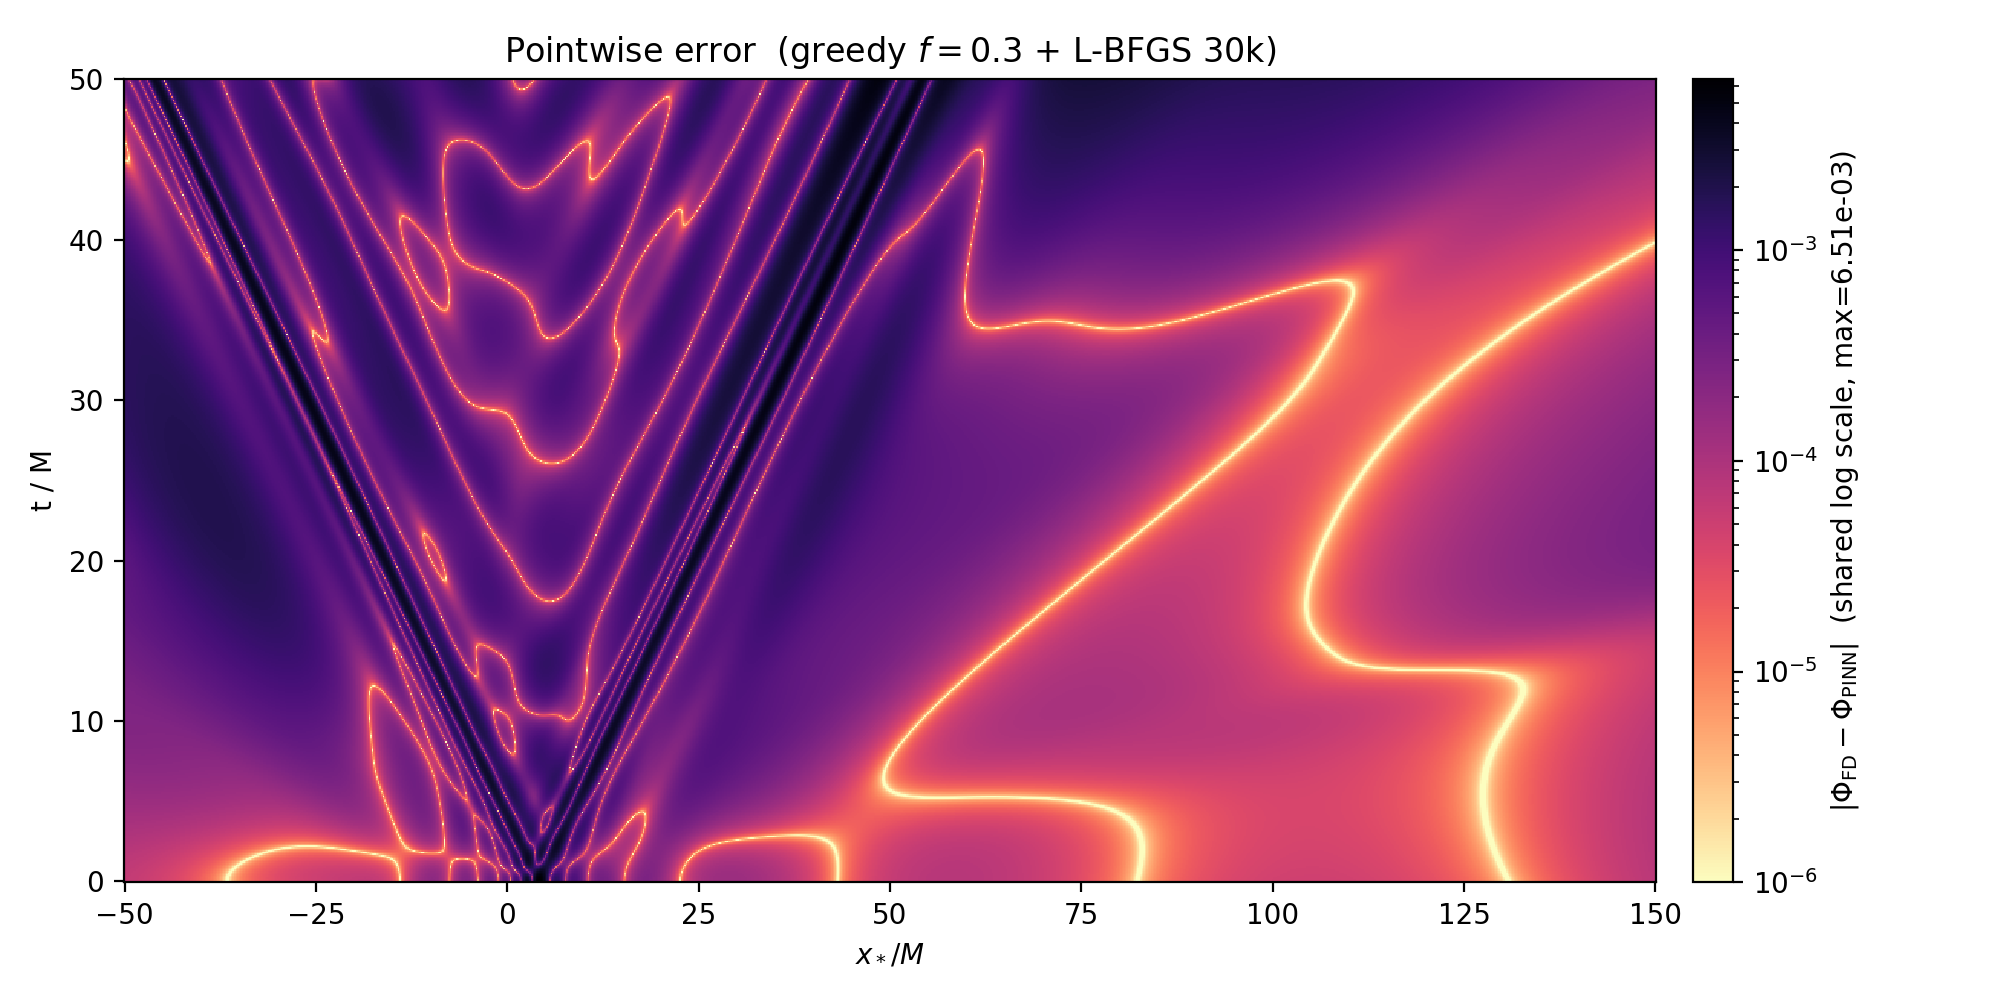
\includegraphics[width=\textwidth,height=0.72\textheight,keepaspectratio]{../outputs/pinn/zerilli_l2_greedy_f03_lbfgs30k/error_heatmap_compare.png}
      \\[2pt]{\scriptsize Greedy $f\!=\!0.3$ + L-BFGS 30k: same colour scale,
      pointwise error reduced by an order of magnitude in the wavefront band.}
    \end{column}
  \end{columns}
\end{frame}


% ══════════════════════════════════════════════════════════════════
\section{7. Summary}
% ══════════════════════════════════════════════════════════════════

\begin{frame}{Summary of the project}
  \begin{enumerate}
    \item \textbf{Problem:} compute Schwarzschild $\ell\!=\!2$ \qnms{}
          from the Zerilli PDE using PINNs --- forward and inverse.
    \medskip
    \item \textbf{Forward PINN best:} greedy $f\!=\!0.3$ + L-BFGS 30k.\\
          $\omega$ to \textbf{0.029\%}, $\tau$ to \textbf{1.99\%}, RMSD
          $-55\%$ vs.\ uniform baseline.
    \medskip
    \item \textbf{Inverse PINN best:} variant D (combo).\\
          $M$ to \textbf{0.34\%}, $\omega$ to \textbf{0.31\%},
          $\tau$ to \textbf{1.59\%} from a single training run.
    \medskip
    \item \textbf{Extraction methodology M3, M4, M5:}\\
          Two-mode templates + plateau scans give principled,
          falsifiable $(\omega, \tau)$ estimates with systematic-error
          bars; M5 is the first systematic 2-D plateau analysis for
          PINN-derived ringdowns.
    \medskip
    \item \textbf{Greedy resampling:} simple, deterministic,
          one-hyperparameter improvement on RAD; now the default.
  \end{enumerate}
\end{frame}

\begin{frame}{Where we are vs.\ where we go next}
  \textbf{Honest scope:}
  \begin{itemize}\small
    \item PINNs cannot beat Leaver on forward Schwarzschild --- Leaver
          is the reference, and the PINN is trained against an FD ground truth.
    \item The contribution is methodological:
          \emph{controlled benchmark} of a class of methods on a problem
          with known answers.
  \end{itemize}
  \medskip
  \textbf{Where it still pays:}
  \begin{itemize}\small
    \item \textbf{Inverse problem:} jointly fit PDE + ringdown data,
          recover $M, \omega, \tau$ in one shot.
    \item \textbf{Differentiable surrogate:} once trained, $\Phi_{\theta}$
          gives free derivatives w.r.t.\ $M$ for downstream inference.
  \end{itemize}
  \medskip
  \textbf{Open directions:}
  \begin{itemize}\small
    \item Multi-mode inverse template (variant E started, $\tau$ to $1.30\%$).
    \item Noisy / short-window inverse: PINN vs.\ Prony/ESPRIT shoot-out.
    \item Kerr ($a \neq 0$) --- two coupled equations, harder ground truth.
  \end{itemize}
\end{frame}

\begin{frame}{}
  \begin{center}
    {\Large Thank you}
    \bigskip\\
    Questions?
  \end{center}
\end{frame}


% ══════════════════════════════════════════════════════════════════
\renewcommand{\mainend}{\inserttotalframenumber}
\makeatletter
\immediate\write\@auxout{\string\gdef\string\mainend{\the\c@framenumber}}
\makeatother

\appendix
\setbeamertemplate{footline}{%
  \hfill\usebeamerfont{footline}Appendix\hspace*{4pt}\vskip4pt%
}

\begin{frame}{Appendix --- Inverse PINN variants ($M$, $\omega$, $\tau$ recovery)}
  \begin{center}\footnotesize
    \begin{tabular}{@{}lcccl@{}}
      \toprule
      \textbf{Variant} & $M$ \textbf{err} & $\omega$ \textbf{err (M4)}
        & $\tau$ \textbf{err (M2 wide)} & \textbf{Change vs.\ baseline} \\
      \midrule
      Baseline                  & 0.41\% & 1.46\%           & 5.27\%        & --- \\
      A: $t_{\text{ring}}^{\min}\!=\!18M$ & 0.45\% & 0.89\%           & \textbf{0.43\%} & later ringdown window \\
      B: $\lambda_{\text{ring}}\!=\!100$ & 1.25\% & nan              & 23.27\%       & ringdown weight up \\
      C: $N_{\text{ring}}\!=\!1000$      & 0.34\% & 50.3\%           & 5.14\%        & more template points \\
      \rowcolor{green!10}
      \textbf{D: A+B+C combined}    & \textbf{0.34\%} & \textbf{0.31\%}  & 1.59\% & headline result \\
      E: two-mode template      & 1.44\% & 2.63\%           & \textbf{1.30\%} & joint fundamental + overtone \\
      \bottomrule
    \end{tabular}
  \end{center}
  \medskip
  \begin{itemize}\small
    \item Single-axis tweaks (A, B, C alone) trade off: each fixes one bias
          and worsens another.
    \item Combined recipe (D) is the only configuration where all three
          parameters are simultaneously below $1.6\%$.
  \end{itemize}
\end{frame}

\begin{frame}{Appendix --- M4 stability scan, inverse PINN}
  \begin{center}
    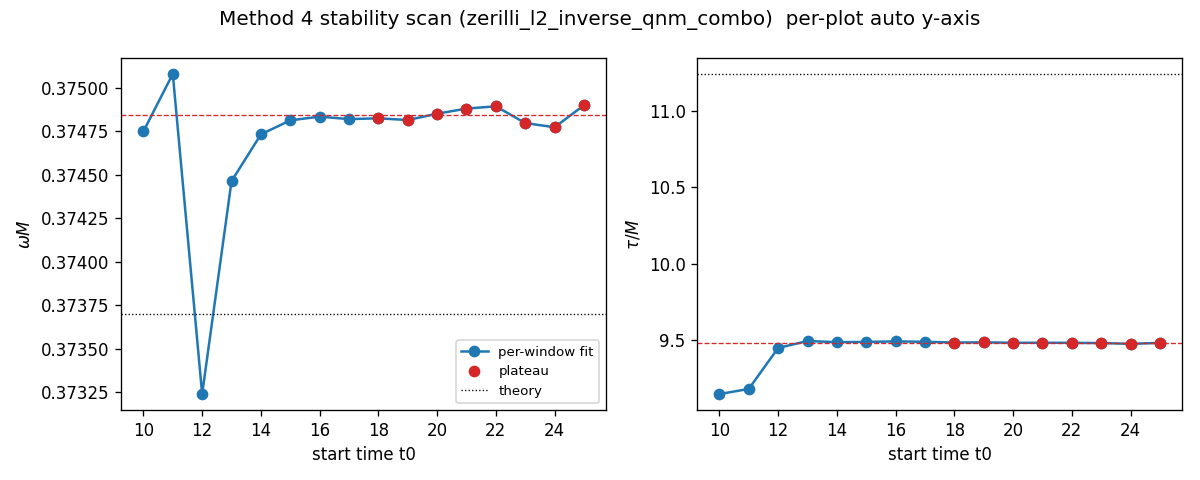
\includegraphics[width=0.62\textwidth]{../outputs/qnm/zerilli_l2_inverse_qnm_combo/pinn_method4_stability.png}
    \\{\footnotesize Variant D inverse PINN: M4 plateau is sharp and narrow
    ($\sigma_{\omega} = 4.4\times10^{-5}$).}
  \end{center}
\end{frame}

\begin{frame}{Appendix --- M5 2-D heatmap, inverse PINN}
  \begin{center}
    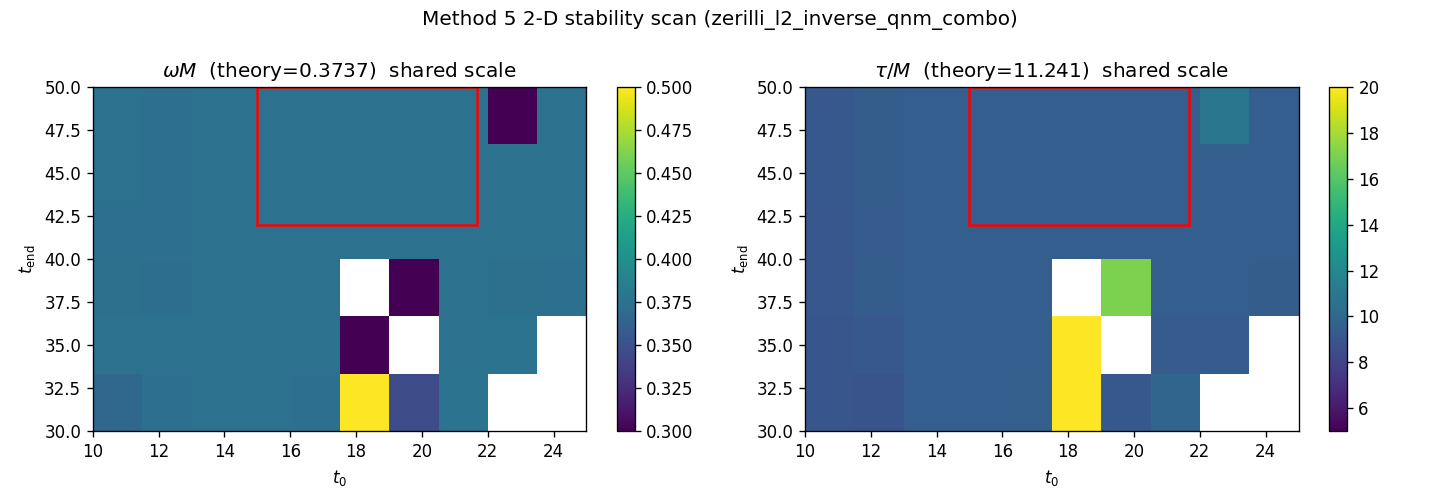
\includegraphics[width=\textwidth,height=0.82\textheight,keepaspectratio]{../outputs/qnm/zerilli_l2_inverse_qnm_combo/pinn_method5_2d_heatmap.png}
    \\{\footnotesize Variant D inverse PINN: M5 confirms a wide stable
    rectangle in the $(t_{0}, t_{\text{end}})$ plane.}
  \end{center}
\end{frame}

\begin{frame}{Appendix --- Greedy vs.\ baseline error heatmaps}
  \begin{columns}[T]
    \begin{column}{0.48\textwidth}
      \centering
      
\includegraphics[width=\textwidth]{../../project32_qnm_pinn/outputs/pinn/zerilli_l2_paper/error_heatmap.png}
      \\{\footnotesize Uniform baseline (Patel et al.\ 2024 reproduction).}
    \end{column}
    \begin{column}{0.48\textwidth}
      \centering
      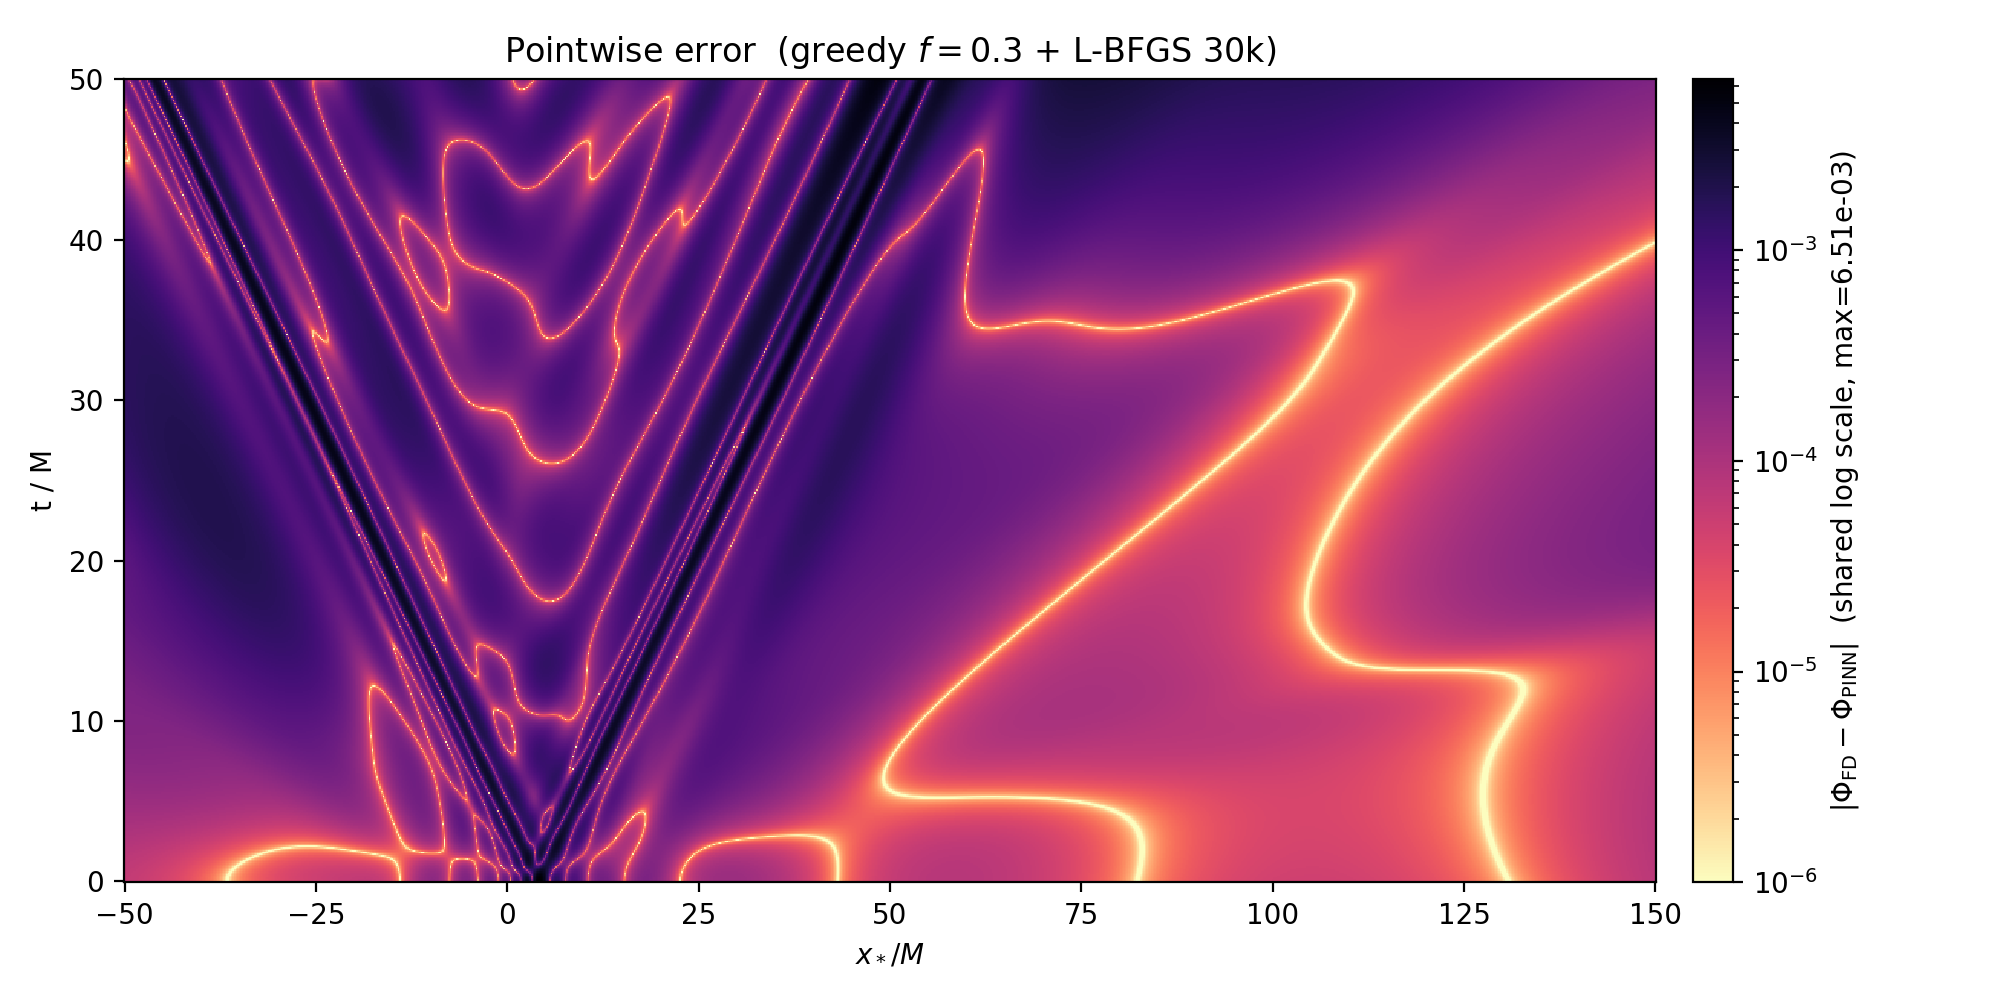
\includegraphics[width=\textwidth]{../outputs/pinn/zerilli_l2_greedy_f03_lbfgs30k/error_heatmap_compare.png}
      \\{\footnotesize Greedy $f\!=\!0.3$ + L-BFGS 30k (best).}
    \end{column}
  \end{columns}
\end{frame}

\begin{frame}{Appendix --- M3 (ESPRIT) algorithm}
  \small
  Given $y[n] = \sum_{k=1}^{K} A_{k}\,z_{k}^{n}$ with $z_{k} = e^{(i\omega_{k}-1/\tau_{k})\Delta t}$:
  \begin{enumerate}
    \item Build Hankel matrix $H \in \mathbb{C}^{(N-L)\times L}$ from $y$.
    \item Truncated SVD: $H = U \Sigma V^{\dagger}$, keep top $K$ columns
          $\Rightarrow$ signal subspace $U_{s}$.
    \item Form $U_{s,1}$ (drop last row), $U_{s,2}$ (drop first row).
    \item Solve $U_{s,1}\Psi = U_{s,2}$ in least squares.
    \item Eigenvalues of $\Psi$ are $\{z_{k}\}$ $\Rightarrow$
          $\omega_{k} = \mathrm{Im}(\log z_{k})/\Delta t$,
          $\tau_{k}^{-1} = -\mathrm{Re}(\log z_{k})/\Delta t$.
    \item Solve a linear least-squares for $\{A_{k}\}$;
          report largest-amplitude mode.
  \end{enumerate}
  \medskip
  \textbf{Conditioning check:} we flag the result as ill-conditioned if
  the dominant amplitude falls below a numerical threshold (here
  $|A| < 10^{-20}$); this catches cases where ESPRIT has fitted noise.
\end{frame}

\end{document}
